\documentclass[a4paper, 12pt]{report}

\usepackage[italian]{babel}
\usepackage{graphicx}
\usepackage{float}
\usepackage{tabularx}
\usepackage{ltablex}
\usepackage[font=small,format=plain,labelfont=bf,up,textfont=normal,up,justification=justified,singlelinecheck=false,skip=0.01\linewidth]{caption}
\renewcommand{\familydefault}{\sfdefault}

\title{"Progetto di una base di dati per la gestione del ciclo di vita del difetto nella produzione dell'elettrodomestico"}
\author{Castellucci Matteo\\Matricola 0000825436\\Anno accademico 2018-2019}
\date{\today}

\begin{document}

\maketitle

\tableofcontents

\chapter{Introduzione}
In questo progetto si vuole realizzare una base di dati a supporto della gestione dei difetti nella realizzazione dell'elettrodomestico,
chiudendo la "catena dell'informazione" tra cliente ed azienda nella fase terminale del ciclo di vita del prodotto. Lo scopo è fornire
all'azienda tutte le informazioni necessarie sugli elettrodomestici una volta arrivati nelle mani del cliente finale, così da poter
ottenere informazioni sul campo per quanto riguarda gli obiettivi attesi e disattesi. In particolar modo, l'attenzione è posta sull'elemento
principe per quanto riguarda l'analisi del comportamento di un bene di consumo: il difetto, in tutti i suoi aspetti. Sarà permesso a tutti gli
attori in gioco, tecnici, telefonisti, analisti dei dati e progettisti, di poter avere una visione a tutto tondo del problema che riguarda
il prodotto: le tempistiche di manifestazione, di risoluzione, il tipo di guasto ed altro ancora. Questo permetterà all'azienda di poter
avere più controllo sullo sviluppo e la messa in produzione di futuri progetti avendo a disposizione più informazioni strategiche.

\chapter{Analisi}

\section{Intervista}
Si vuole realizzare una base di dati che permetta di gestire tutte le informazioni che riguardano un guasto di un elettrodomestico.
L'azienda riceve telefonate da un cliente che vengono smistate ad un adeguato centro assistenza dove ciascuna verrà raccolta da un operatore.
Ogni centro assistenza ha sede in una città e possiede una determinata area di competenza, per cui tutte le chiamate che verranno effettuate
all'interno di quest'ultima verranno redirette al centro assistenza associato. L'identificazione dei centri assistenza viene fatta mediante dei
codici che hanno però valenza solamente nazionale.\newline
L'operatore, di cui l'azienda conosce dati identificativi come nome, cognome, data e luogo di nascita, codice fiscale, luogo di residenza, nonché lo 
stipendio che gli elargisce e lo identifica mediante un codice, così come per ogni suo dipendente, chiede al cliente di identificarsi. Vengono richiesti dall'operatore 
il nome, il cognome e il recapito a cui fare riferimento nel momento nel quale un solo tecnico si recherà in loco per riparare il suo elettrodomestico. 
Eventualmente, l'operatore chiede anche l'indirizzo \textit{email}, qualora il cliente lo possieda. Inoltre, viene registrato il numero di telefono 
chiamante a cui verrà fatto riferimento anche in futuro come specifico per quel dato cliente.\newline
In seguito, l'operatore chiede quale prodotto o quali prodotti del cliente hanno subito un guasto e saranno l'oggetto della corrente richiesta di 
assistenza. L'operatore per ogni elettrodomestico ne chiede la categoria, il modello, specificato con un codice, e si fa leggere "PNC" (\textit{Product 
Number Code}) e "SNC" (\textit{Serial Number Code}), codici che lo identificano univocamente trattenendo informazioni sulle caratteristiche tecniche e
la data di produzione. L'operatore richiede inoltre la data di acquisto dell'elettrodomestico e la data di installazione dello stesso e le registra qualora 
il cliente le abbia a disposizione o se ne ricordi. In assenza di data di acquisto sarà compito del tecnico, una volta recatosi a casa del cliente, 
recuperare almeno questa informazione e in caso la garanzia del prodotto sia scaduta o non sia trovata, far pagare il cliente. Il cliente potrebbe avere 
aderito opzionalmente ad un programma di estensione della garanzia, identificato da un codice, informazione che deve fornire, se non fase in chiamata, 
almeno al momento della visita. Da ultimo, l'operatore chiede al cliente di farsi descrivere il guasto o i guasti subiti e registra la data corrente come data di apertura 
della pratica, ponendo lo stato dell'intervento come aperto e concorda con il cliente la data di visita del tecnico a casa per la riparazione.\newline
Un difetto è univocamente determinato da due codici, il "\textit{Component Code}", che identifica quale parte di un elettrodomestico viene affetto, e
il codice di tipo, che indica qual è nello specifico il tipo di difetto che il componente può subire. Ad ogni difetto sono associati i ricambi che sono 
necessari per poterlo sistemare, che potrebbero anche essere più di uno o nessuno, identificati da un codice, e il costo di ciascuno di essi, 
sia in termini di costo del ricambio stesso, che del costo di manodopera per l'installazione.\newline
Un tecnico, che afferisce ad un centro assistenza come l'operatore, si preoccuperà, una volta raccolte le informazioni necessarie dalla chiamata,
di recarsi a casa del cliente e registrare a sua volta una descrizione personale del guasto o dei guasti del cliente, dopodiché possibilmente li riparerà
e si preoccuperà di chiudere la richiesta di assistenza pendente. Specificherà anche il tempo che ha impiegato nel risolvere il problema del cliente
espresso in quarti d'ora. Un tecnico può lavorare direttamente per l'azienda o è assunto tramite un'impresa terza per l'azienda stessa. \newline
Un progettista di elettrodomestici dovrà poi periodicamente recuperare le informazioni riguardanti i guasti che si sono verificati sui prodotti che
gli competono, indicati dalla o dalle categorie di prodotto a cui è assegnato, e stilare classifiche che possano aiutare l'azienda a migliorare la produzione.

\section{Analisi ed eliminazione delle ambiguità}

\begin{tabularx}{\linewidth}{X|X}
	\hline
	\textbf{Termine presente nel testo} & \textbf{Sinonimo utilizzato}\\
	\hline
	\hline
	Elettrodomestico & Prodotto\\
	\hline
	Pratica & Intervento\\
	\hline
	Telefonata & Intervento\\
	\hline
	Richiesta di assistenza & Intervento\\
	\hline
	Chiamata & Intervento\\
	\hline
	Riparazione & Intervento\\
	\hline
	\caption{Associazioni termine-sinonimo per formulare specifiche non ambigue}
\end{tabularx}

Il termine "elettrodomestico" verrà da qui in avanti sostituito dal termine "prodotto", in quanto dotato di una più adeguato carattere di astrattezza
e generalità, benché il caso in esame sia studiato su di un'azienda che produce elettrodomestici. I termini come "chiamata", "richiesta di
assistenza", "intervento" e loro sinonimi vengono tutti raccolti sotto il termine "intervento" poiché di fatto descrivono le varie fasi dello
stesso, dalla richiesta iniziale del cliente, alla visita del tecnico dell'assistenza, fino alla riparazione del prodotto indicato. Si intende
che ogni intervento sarà raccolto in un'unica pratica e perciò anche quest'ultimo termine indica lo stesso concetto.

\section{Definizione delle specifiche ed estrapolazione dei concetti}
Si vuole realizzare una base di dati che permetta di gestire tutte le informazioni che riguardano un \textbf{guasto} di un \textbf{prodotto}.
Un prodotto è univocamente identificato da una combinazione di codici detti "PNC" (\textit{Product Number Code}) e "SNC" (\textit{Serial Number Code}) ed è caratterizzato
da una \textbf{categoria} e un \textbf{modello} sotto forma di codice. Un prodotto possiede inoltre una data di acquisto e una di installazione, insieme ad 
un'\textbf{estensione di garanzia} identificata da un codice, informazioni che però possono essere disponibili o meno, a seconda che il \textbf{cliente}
che lo possiede ne abbia tenuto traccia o meno.\newline
Al verificarsi di un guasto, il cliente si preoccupa di chiamare l'assistenza clienti dell'azienda produttrice per richiedere un
\textbf{intervento}. Ogni cliente verrà identificato dal suo numero di telefono e verranno registrati il suo nome, il suo cognome,
il recapito presso il quale inviare il \textbf{tecnico} per la riparazione del prodotto ed opzionalmente il suo indirizzo \textit{email},
solamente nel caso il cliente lo possedesse.\newline
Il cliente parlerà con un \textbf{operatore}, che chiederà al cliente tutte le informazioni relative al prodotto o ai prodotti
che hanno subito un guasto insieme alle descrizioni dei guasti stessi che vengono anch'esse registrate. Viene inoltre concordata una data di
visita del tecnico affinché possa riparare il prodotto. Infine, vengono registrati la data della chiamata del cliente e viene
aggiornato lo stato dell'intervento come aperto. Quando il tecnico visiterà il cliente, uno solo per intervento, registrerà una sua descrizione
del guasto per ognuno di essi e dopo averli riparati segnerà lo stato dell'intervento come chiuso. Indicherà anche il tempo speso per farlo in quarti d'ora.\newline
Un guasto è associato ad uno specifico \textbf{difetto}, il quale è univocamente determinato da due codici: il "\textit{Component Code}"
che identifica il \textbf{componente} del prodotto coinvolto e un codice che identifica il tipo del difetto su quello specifico componente. Nella
riparazione di un difetto possono essere utilizzati uno o più \textbf{ricambi}, ognuno dei quali è identificato da un codice e vi è associato
sia un costo di acquisto per il ricambio stesso che di manodopera per l'installazione.\newline
L'azienda possiede per i suoi dipendenti informazioni come il codice fiscale, il nome, il cognome, la data e il luogo di nascita, luogo di
residenza e lo stipendio percepito e li identifica mediante un codice. I dipendenti presi in considerazione sono gli operatori, i tecnici e i
\textbf{progettisti}. Gli operatori e i tecnici afferiscono ad uno specifico \textbf{centro assistenza} dell'azienda,
mentre i progettisti sono interessati ad analizzare i dati dei guasti di una o più categorie di prodotto stilando delle classifiche. Un tecnico
inoltre può essere dipendente interno dell'azienda oppure no.\newline
Un centro assistenza ha sede in una città e possiede una determinata area di competenza, nella quale tutte le telefonate che vengono fatte
per l'assistenza vengono inoltrate a quello specifico centro. Esso è identificato da un codice univoco, ma solo nella nazione in cui si trova.\newline

\begin{tabularx}{\linewidth}{>{\hsize=0.375\hsize}X|X|>{\hsize=0.475\hsize}X}
	\hline
	\textbf{Termine} & \textbf{Descrizione} & \textbf{Collegamenti}\\
	\hline
	\hline
	Prodotto & Un elettrodomestico di un determinato modello che l'azienda ha rilasciato sul mercato ed è stato comprato da un cliente, per poi subire un guasto &
	Cliente,\newline Modello,\newline Guasto\\
	\hline
	Modello & Una classe di prodotti accomunata da caratteristiche comuni & Prodotto\\
	\hline
	Cliente & Una persona che ha acquistato un prodotto presso l'azienda e ha richiesto un intervento per quello specifico prodotto & Prodotto,\newline 
	Intervento\\
	\hline
	Guasto & Un problema di varia natura che si è verificato in uno specifico prodotto, causato da un difetto nel prodotto stesso, per cui viene
	richiesto un intervento. Sarà analizzato da un progettista & Prodotto,\newline Difetto,\newline Intervento,\newline Progettista\\
	\hline
	Intervento & Una richiesta fatta da un cliente per risolvere uno o più guasti subiti, sarà registrato da un operatore e risolto da un tecnico
	& Guasto,\newline Operatore,\newline Tecnico\\
	\hline
	Difetto & Una classe di guasti accomunati dal componente in cui il guasto si verifica e la natura del difetto stesso, possono essere utilizzati
	dei ricambi per poterlo riparare & Guasto,\newline Componente,\newline Ricambio\\
	\hline
	Componente & Una parte di un prodotto che può subire un guasto per un suo difetto di produzione & Guasto,\newline Difetto\\
	\hline
	Ricambio & Un componente di un prodotto che può essere utilizzato nella riparazione di un difetto & Prodotto,\newline Difetto\\
	\hline
	Operatore & Un dipendente dell'azienda che si preoccupa di aprire richieste di intervento, appartiene ad un determinato centro assistenza
	& Intervento,\newline Centro Assistenza\\
	\hline
	Tecnico & Un dipendente dell'azienda che si preoccupa di attendere ad interventi di manutenzione e chiudere le richieste pendenti, appartiene
	ad un centro assistenza & Intervento,\newline Centro Assistenza\\
	\hline
	Progettista & Un dipendente dell'azienda che si preoccupa di analizzare i dati sui guasti accaduti, ma solamente su alcuni tipi
	di prodotto & Guasto, Prodotto\\
	\hline
	Centro Assistenza & Parte dell'azienda volta all'impiego di operatori e tecnici di assistenza & Operatore,\newline Tecnico\\
	\hline
	Categoria & Un'insieme di prodotti che rappresentano lo stesso tipo di elettrodomestico (ad esempio: "Forno", "Lavatrice", ecc.) & Prodotto\\
	\hline
	Estensione di garanzia & Particolare programma che può essere scelto per un prodotto per prolungare il periodo per il quale si trova in garanzia & Prodotto\\
	\hline
	\caption{Glossario dei termini}
\end{tabularx}

\chapter{Analisi concettuale}

\section{Schema scheletro}

\begin{figure}[H]
	\centering
	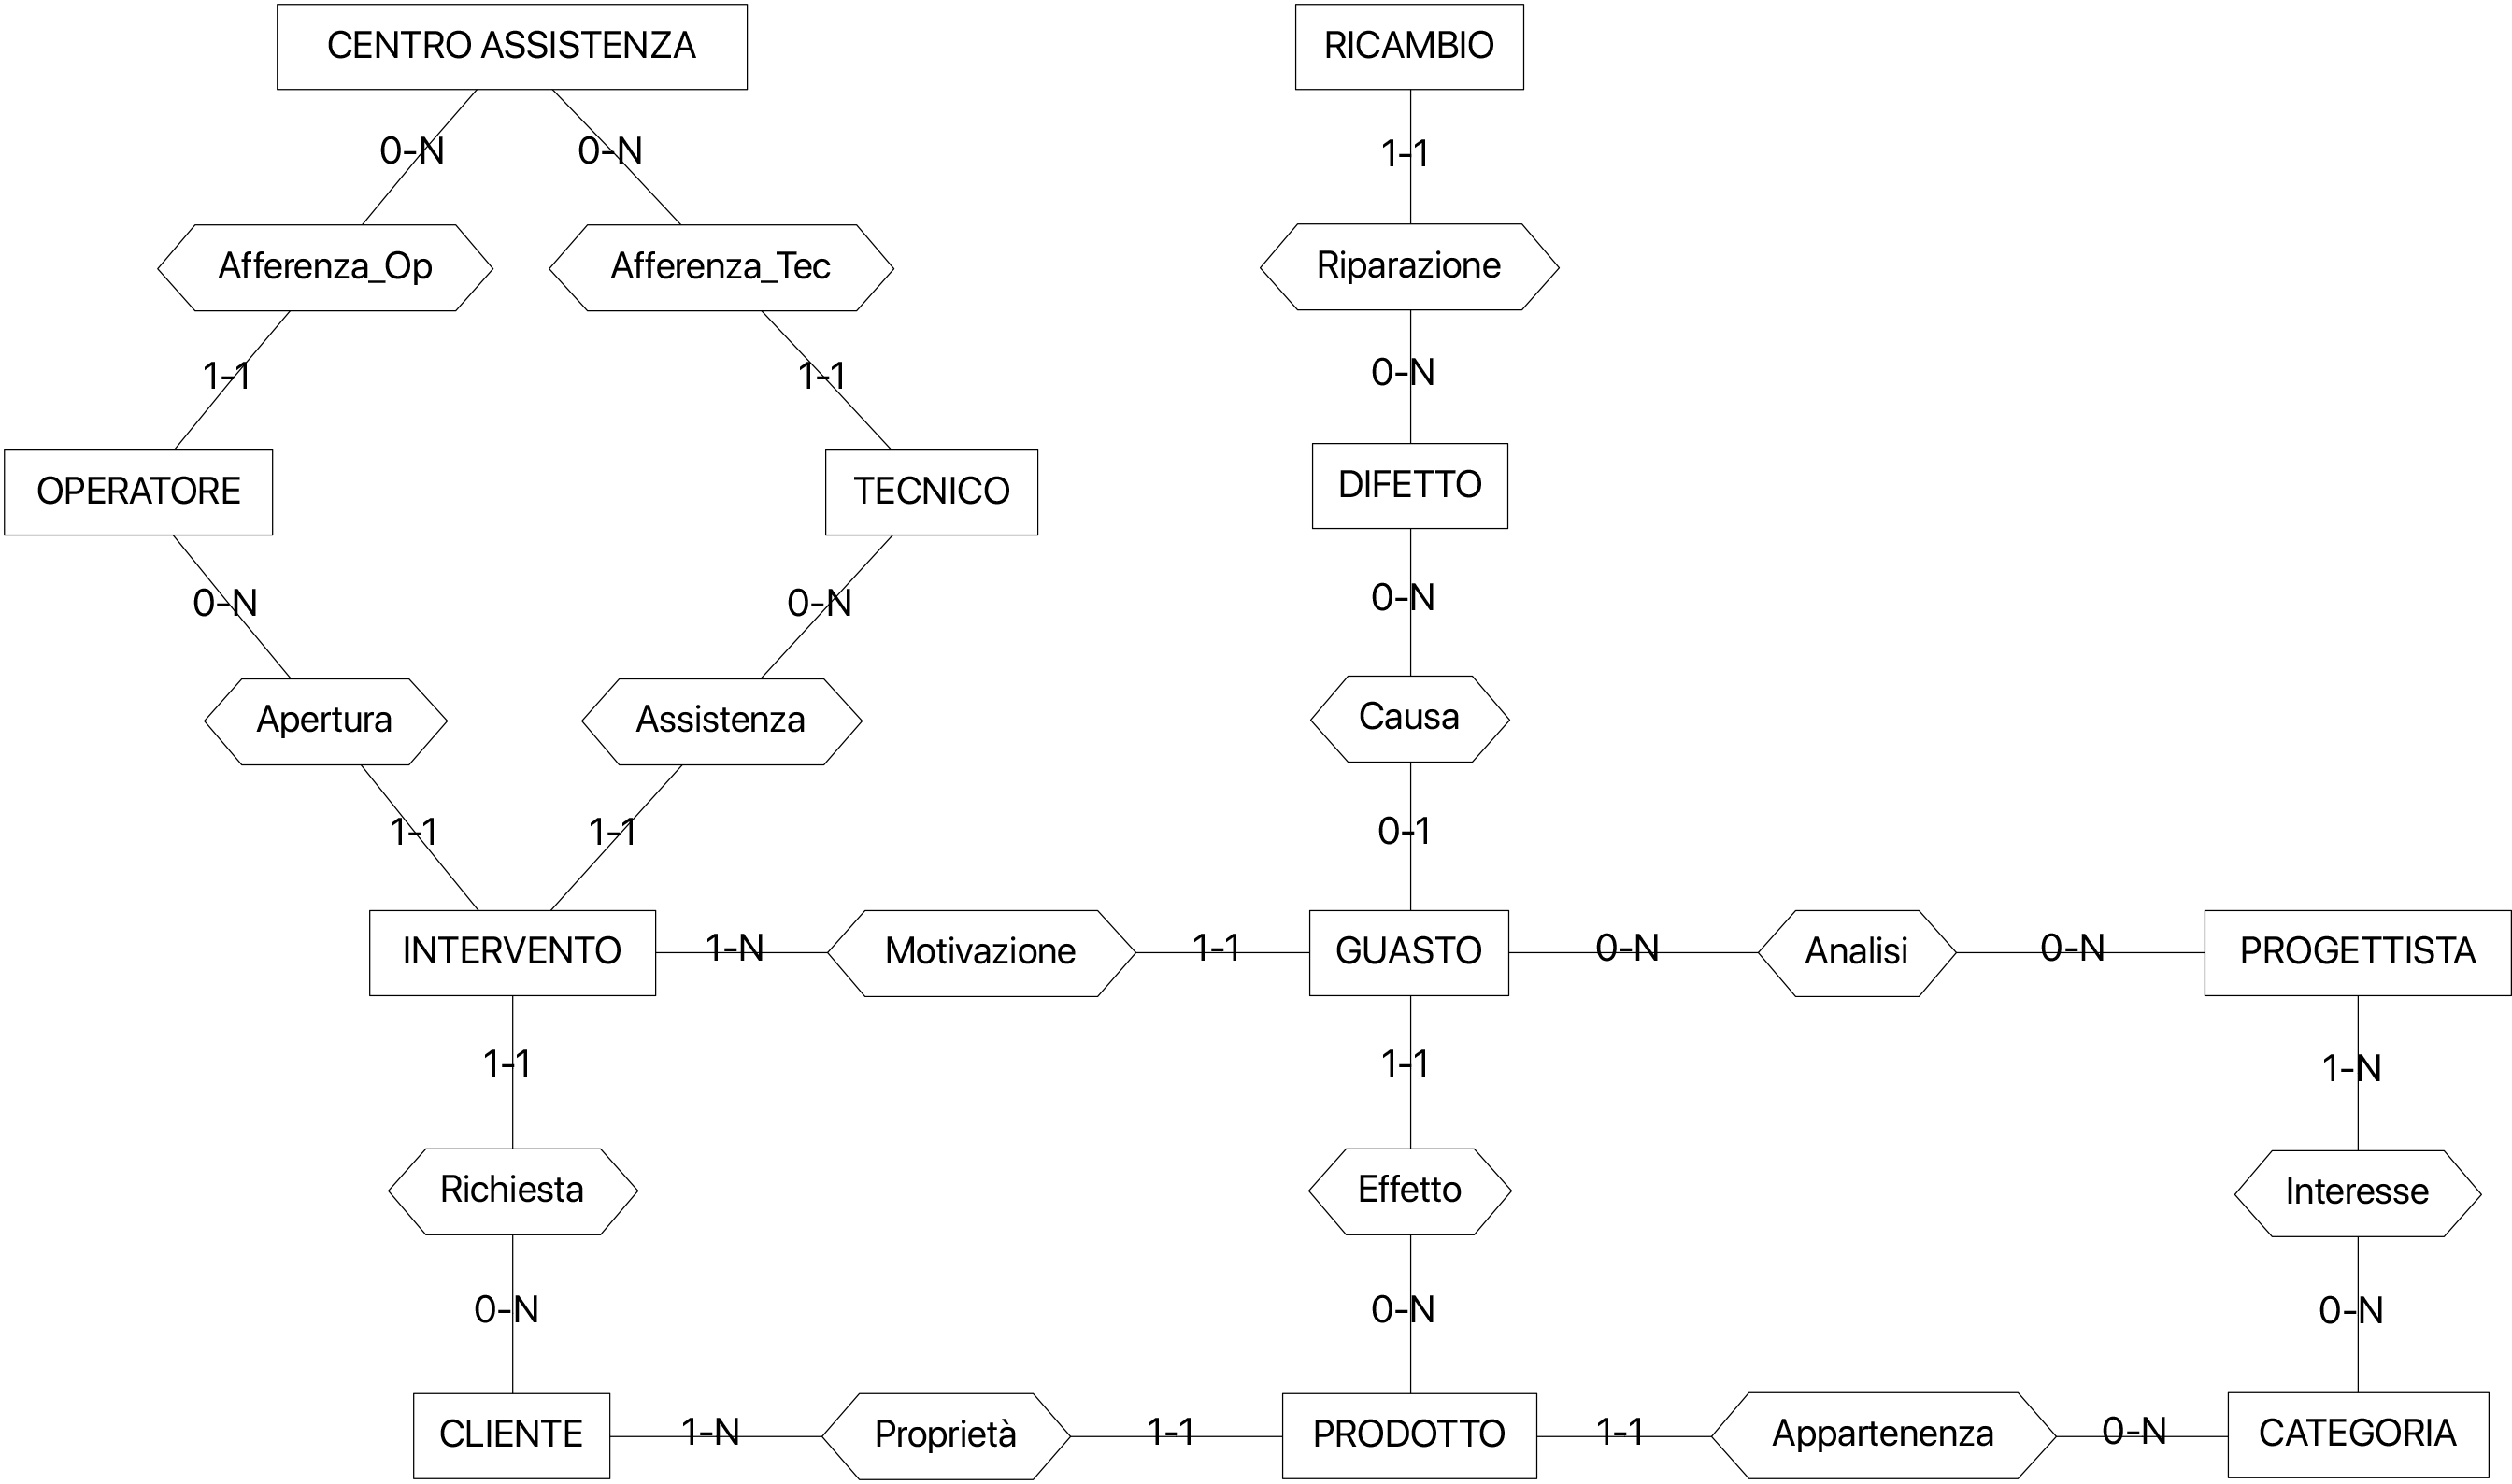
\includegraphics[width=\linewidth]{images/skeleton.png}
	\caption{Schema scheletro dei concetti più rilevanti estrapolati dalle specifiche}
\end{figure}

\section{Raffinamenti proposti}

\subsection{Gerarchia di persone}

Nelle specifiche sono specificati quattro concetti - "cliente", "operatore", "tecnico" e "progettista" - che si prestano a diventare entità, ma
che ruotano tutte attorno alla nozione di persona. Tutte queste infatti sono persone e in quanto tali condividono almeno informazioni come il nome
ed il cognome; è perciò significativo metterle assieme in una gerarchia che discende da persona. Inoltre, tutti e tre i concetti meno che "cliente"
sono di fatto dipendenti dell'azienda e in quanto tali le informazioni che l'azienda trattiene su di essi sono le stesse, pur intrattenendo con gli
altri concetti rapporti diversi a seconda della mansione che svolgono. Anche per queste tre concetti è opportuno raccoglierli attraverso una seconda
gerarchia che origini da dipendente, che a sua volta è una persona. I concetti di "operatore" e "tecnico" saranno poi legati a "centro assistenza"
così come individuato nello schema scheletro. Il "progettista", poiché può occuparsi o di una o di più categorie di prodotto quando analizza i "guasti",
queste gli verranno associate mediante un attributo multiplo obbligatorio. Pur essendo condivise tra più "progettisti" e anche dai "prodotti" stessi,
non è il caso separare il concetto di "categoria" in un'entità a sè stante, perché non presenta nessuna caratteristica che non sia il suo nome stesso
e in caso l'insieme dei prodotti che presentano una stessa categoria dovesse essere rimosso, non è problematico. Infatti, significherebbe semplicemente
che l'azienda ha deciso di voler smettere di trattare le informazioni su una determinata categoria di elettrodomestici e a maggior ragione anche la
categoria stessa è bene che non lasci traccia nel \textit{database}.

\begin{figure}[H]
	\centering
	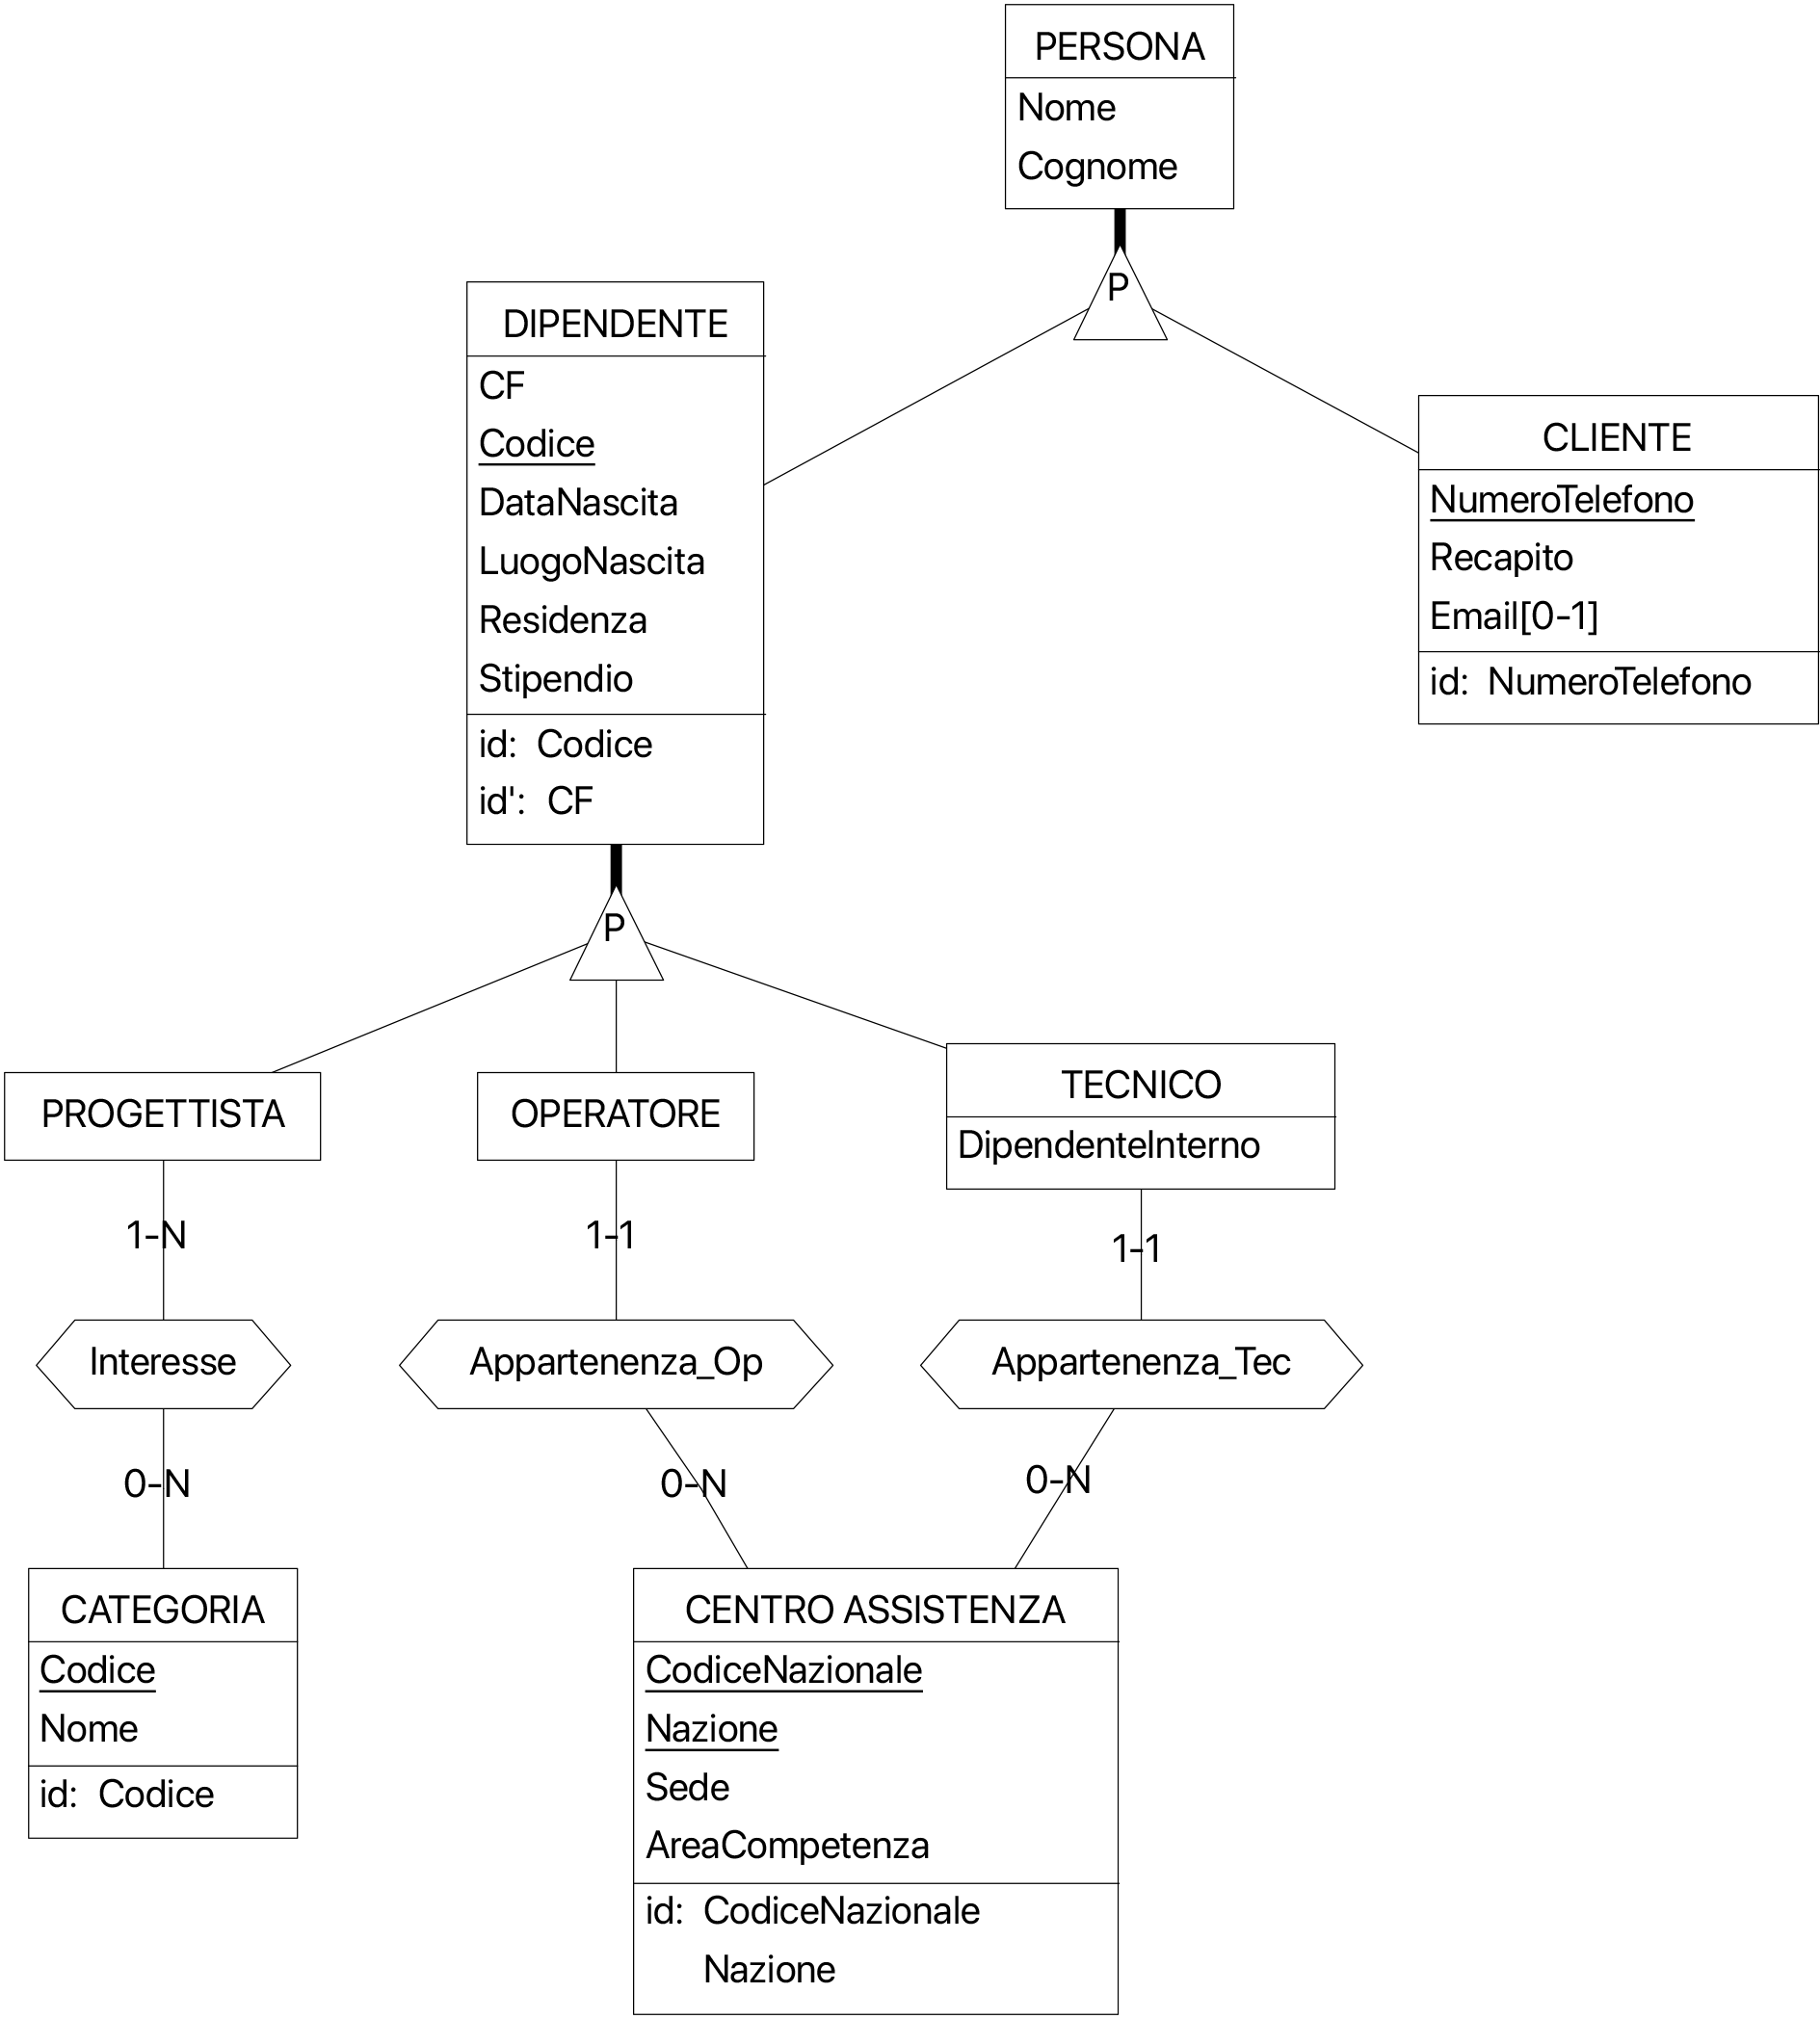
\includegraphics[width=\linewidth]{images/persone.png}
	\caption{Schema raffinato dei concetti riguardanti "persone"}
\end{figure}

\subsection{Necessità di un entità separata per i guasti}

Dai concetti di "persone" è poi immediato spostarsi sui quelli di "intervento" e "guasto" che li coinvolgono più direttamente. Benché il testo
specifichi che siano i prodotti, a causa dei loro guasti, ad essere in numero di uno o più presenti in un intervento, è più adatto frapporre il
concetto di "guasto" tra essi e quello di "intervento". È infatti facile immaginare come un cliente potrebbe voler riportare la presenza
di un guasto solamente dopo che un secondo si è verificato, magari perché il primo non era così urgente, e lo farebbe all'interno dello stesso intervento.
Se eliminassimo il concetto di "guasto" questo non sarebbe possibile e inoltre provocherebbe problemi anche con la nozione di "difetto". Essendo
un prodotto caratterizzato anche da più guasti, infatti, potrebbero essere più di uno i difetti legati ad un prodotto, anche ripetuti nel tempo,
ma una schematizzazione del genere impedirebbe proprio la loro ripetizione. Potrebbe ad esempio verificarsi un guasto diverso in un momento successivo,
che verrà incluso poi in un intervento successivo, ma la cui origine è sempre lo stesso difetto di progettazione.\newline I dati che sono di competenza del tecnico
inserire sono tutti modellati mediante attributi opzionali, poiché si suppone che l'apertura della pratica coincida con l'inserimento di un nuovo
\textit{record} nel \textit{database}, momento nel quale questi dati sono ancora sconosciuti. Per le nozioni di "componente" e "garanzia" è stato
deciso di non renderle entità poiché non possiedono caratteristiche interessanti che non siano i codici stessi che le identificano. Inoltre, un componente
è esso stesso un ricambio, solo acquistato in un secondo momento dalla costruzione dell'elettrodomestico.

\begin{figure}[H]
	\centering
	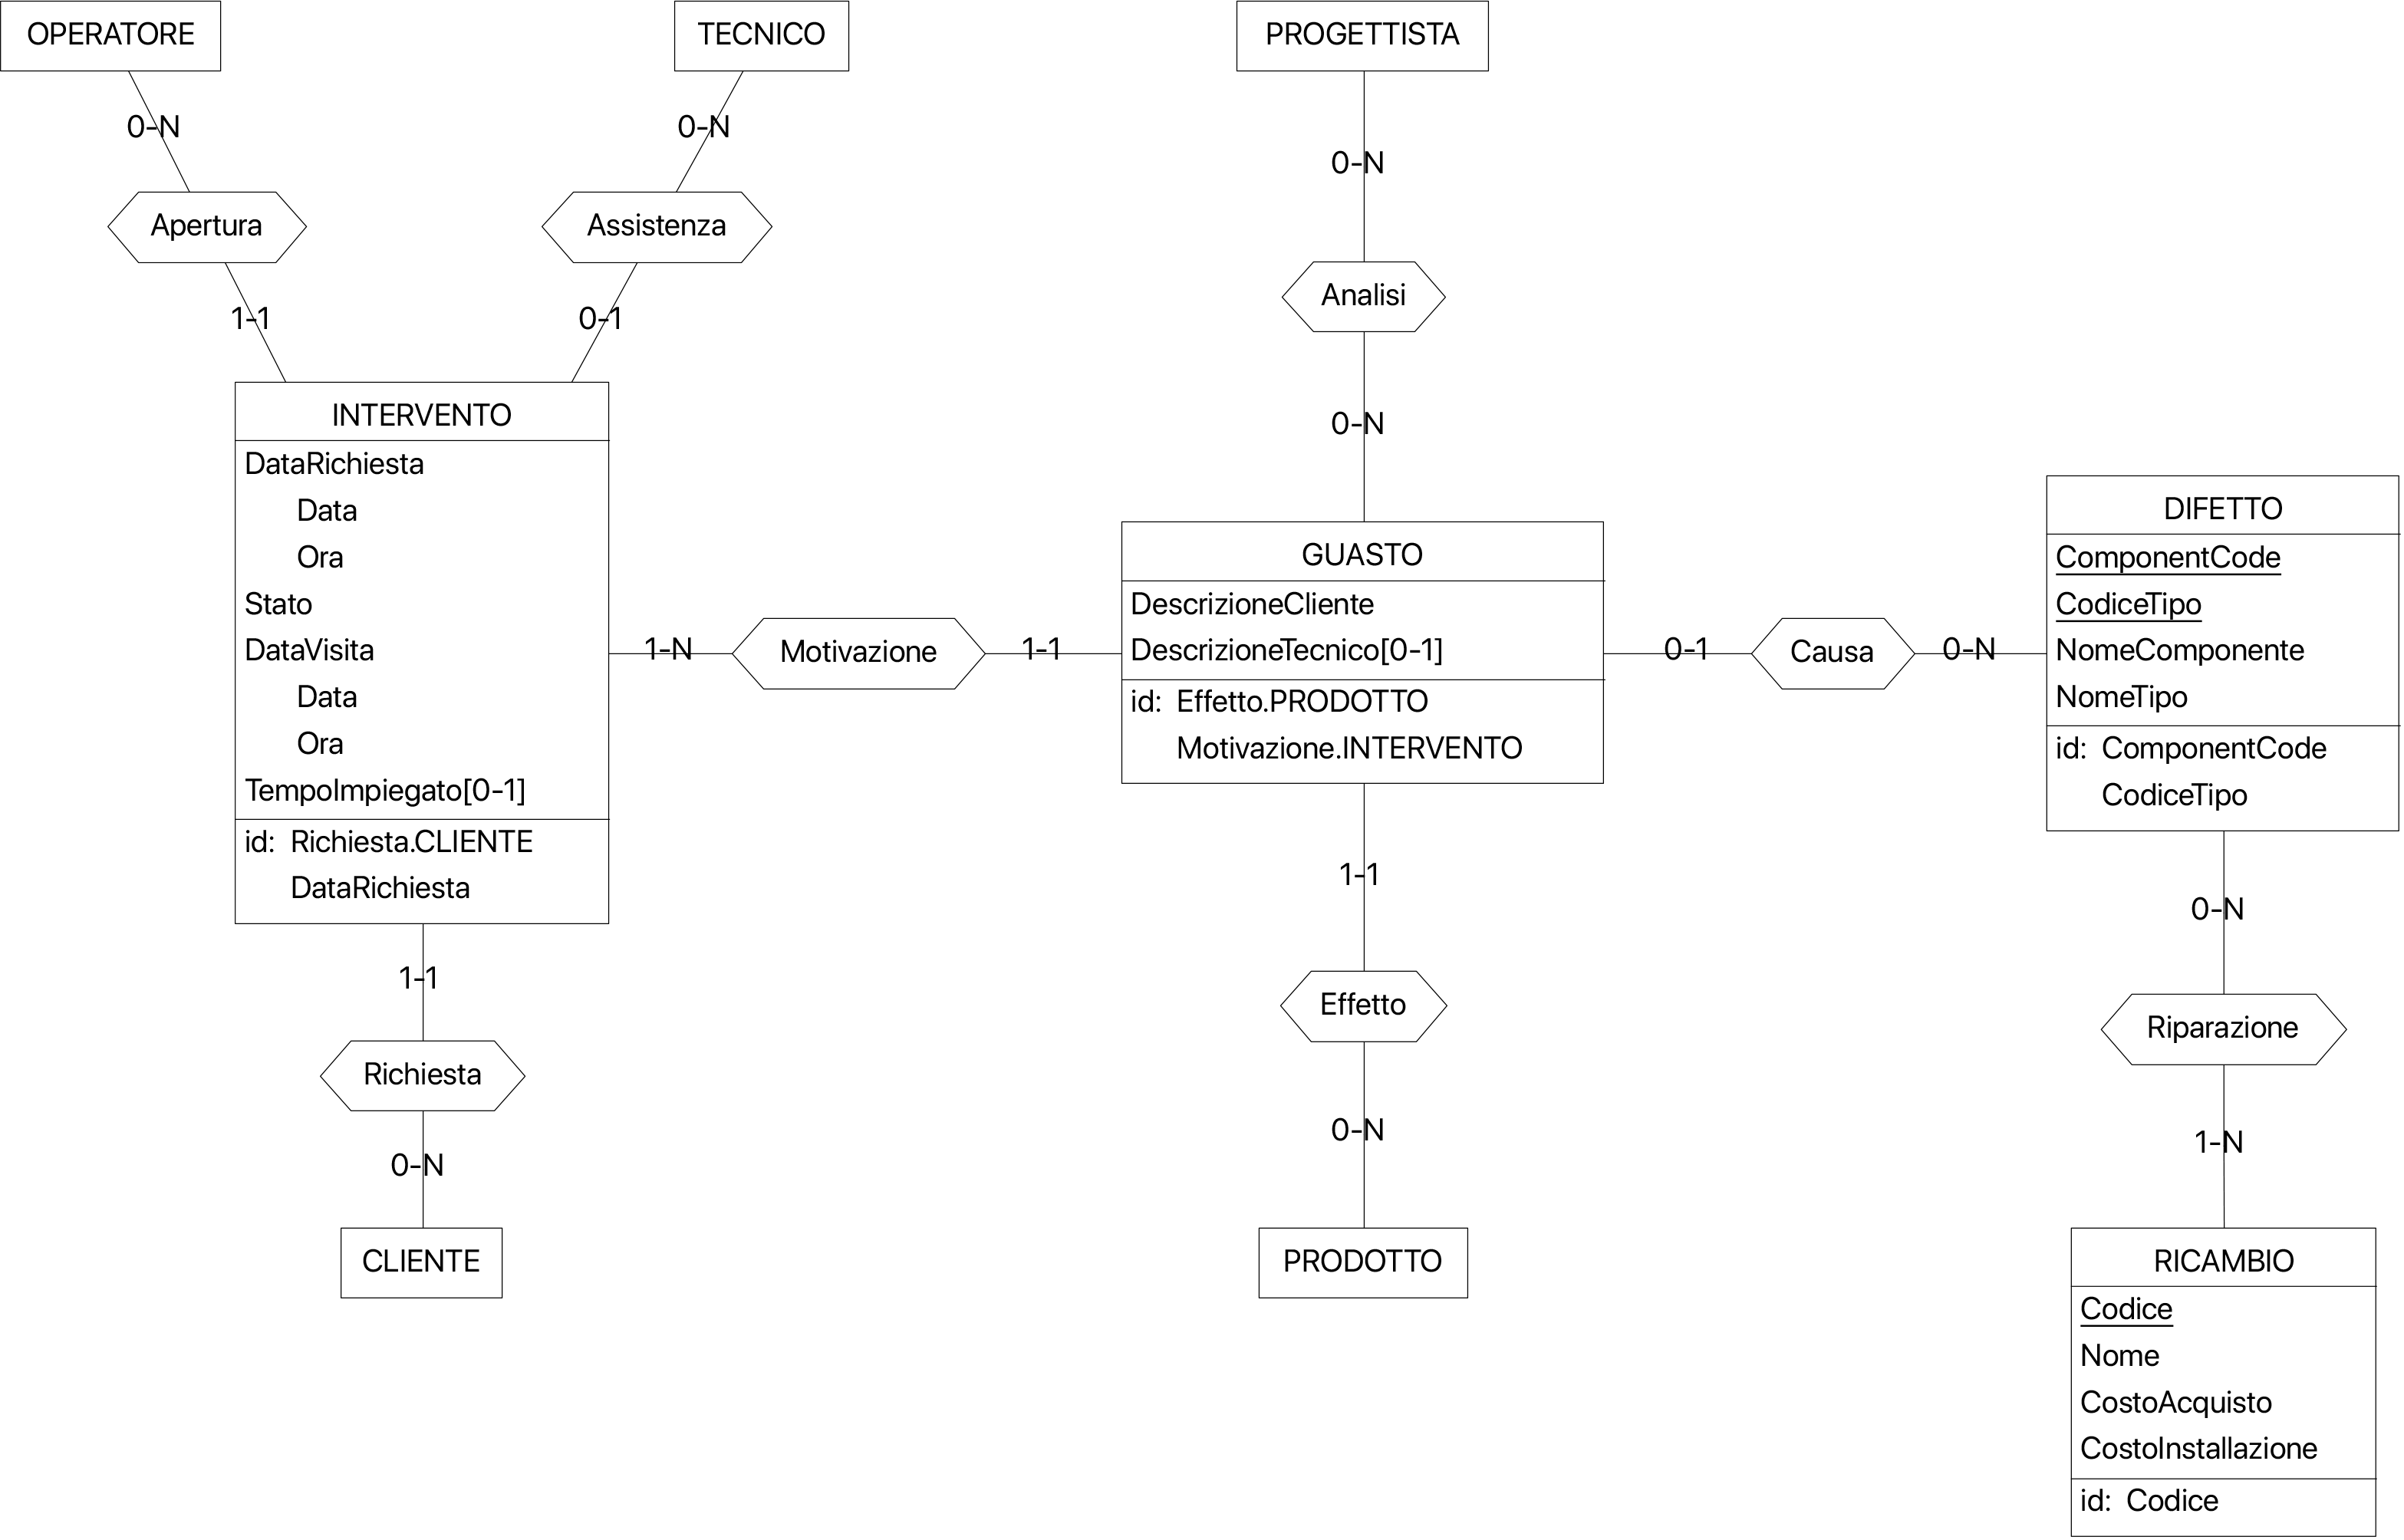
\includegraphics[width=\linewidth]{images/interventi.png}
	\caption{Schema raffinato dei concetti "intervento", "guasto" e "difetto"}
\end{figure}

\subsection{Modellazione del concetto di "prodotto"}

Da ultimo, espandiamo la nozione di "prodotto". Non è una componente dello schema particolarmente significativa, anche se presenta alcune particolarità.
Il fatto che il cliente possa non avere a disposizione le informazioni riguardanti la data di acquisto, installazione o addirittura la garanzia sul
prodotto, richiede una modellazione specifica. In particolar modo, queste informazioni sarà necessario modellarle come attributi singoli opzionali.

\begin{figure}[H]
	\centering
	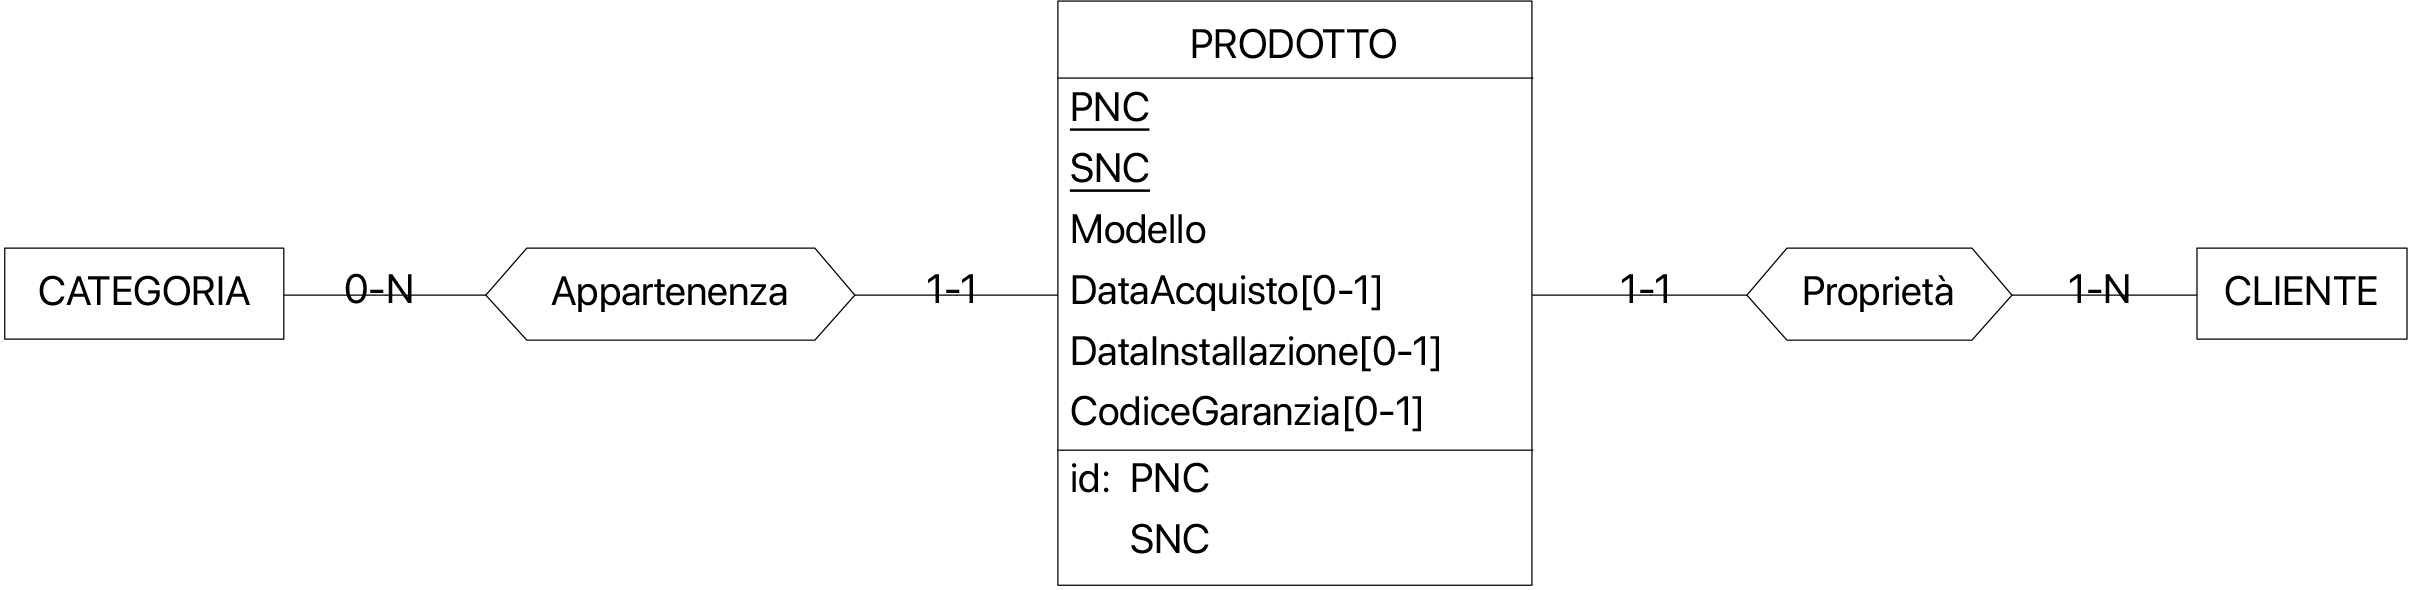
\includegraphics[width=\linewidth]{images/prodotti.png}
	\caption{Schema raffinato del concetto "prodotto" e "modello"}
\end{figure}

\section{Schema finale}

\begin{figure}[H]
	\centering
	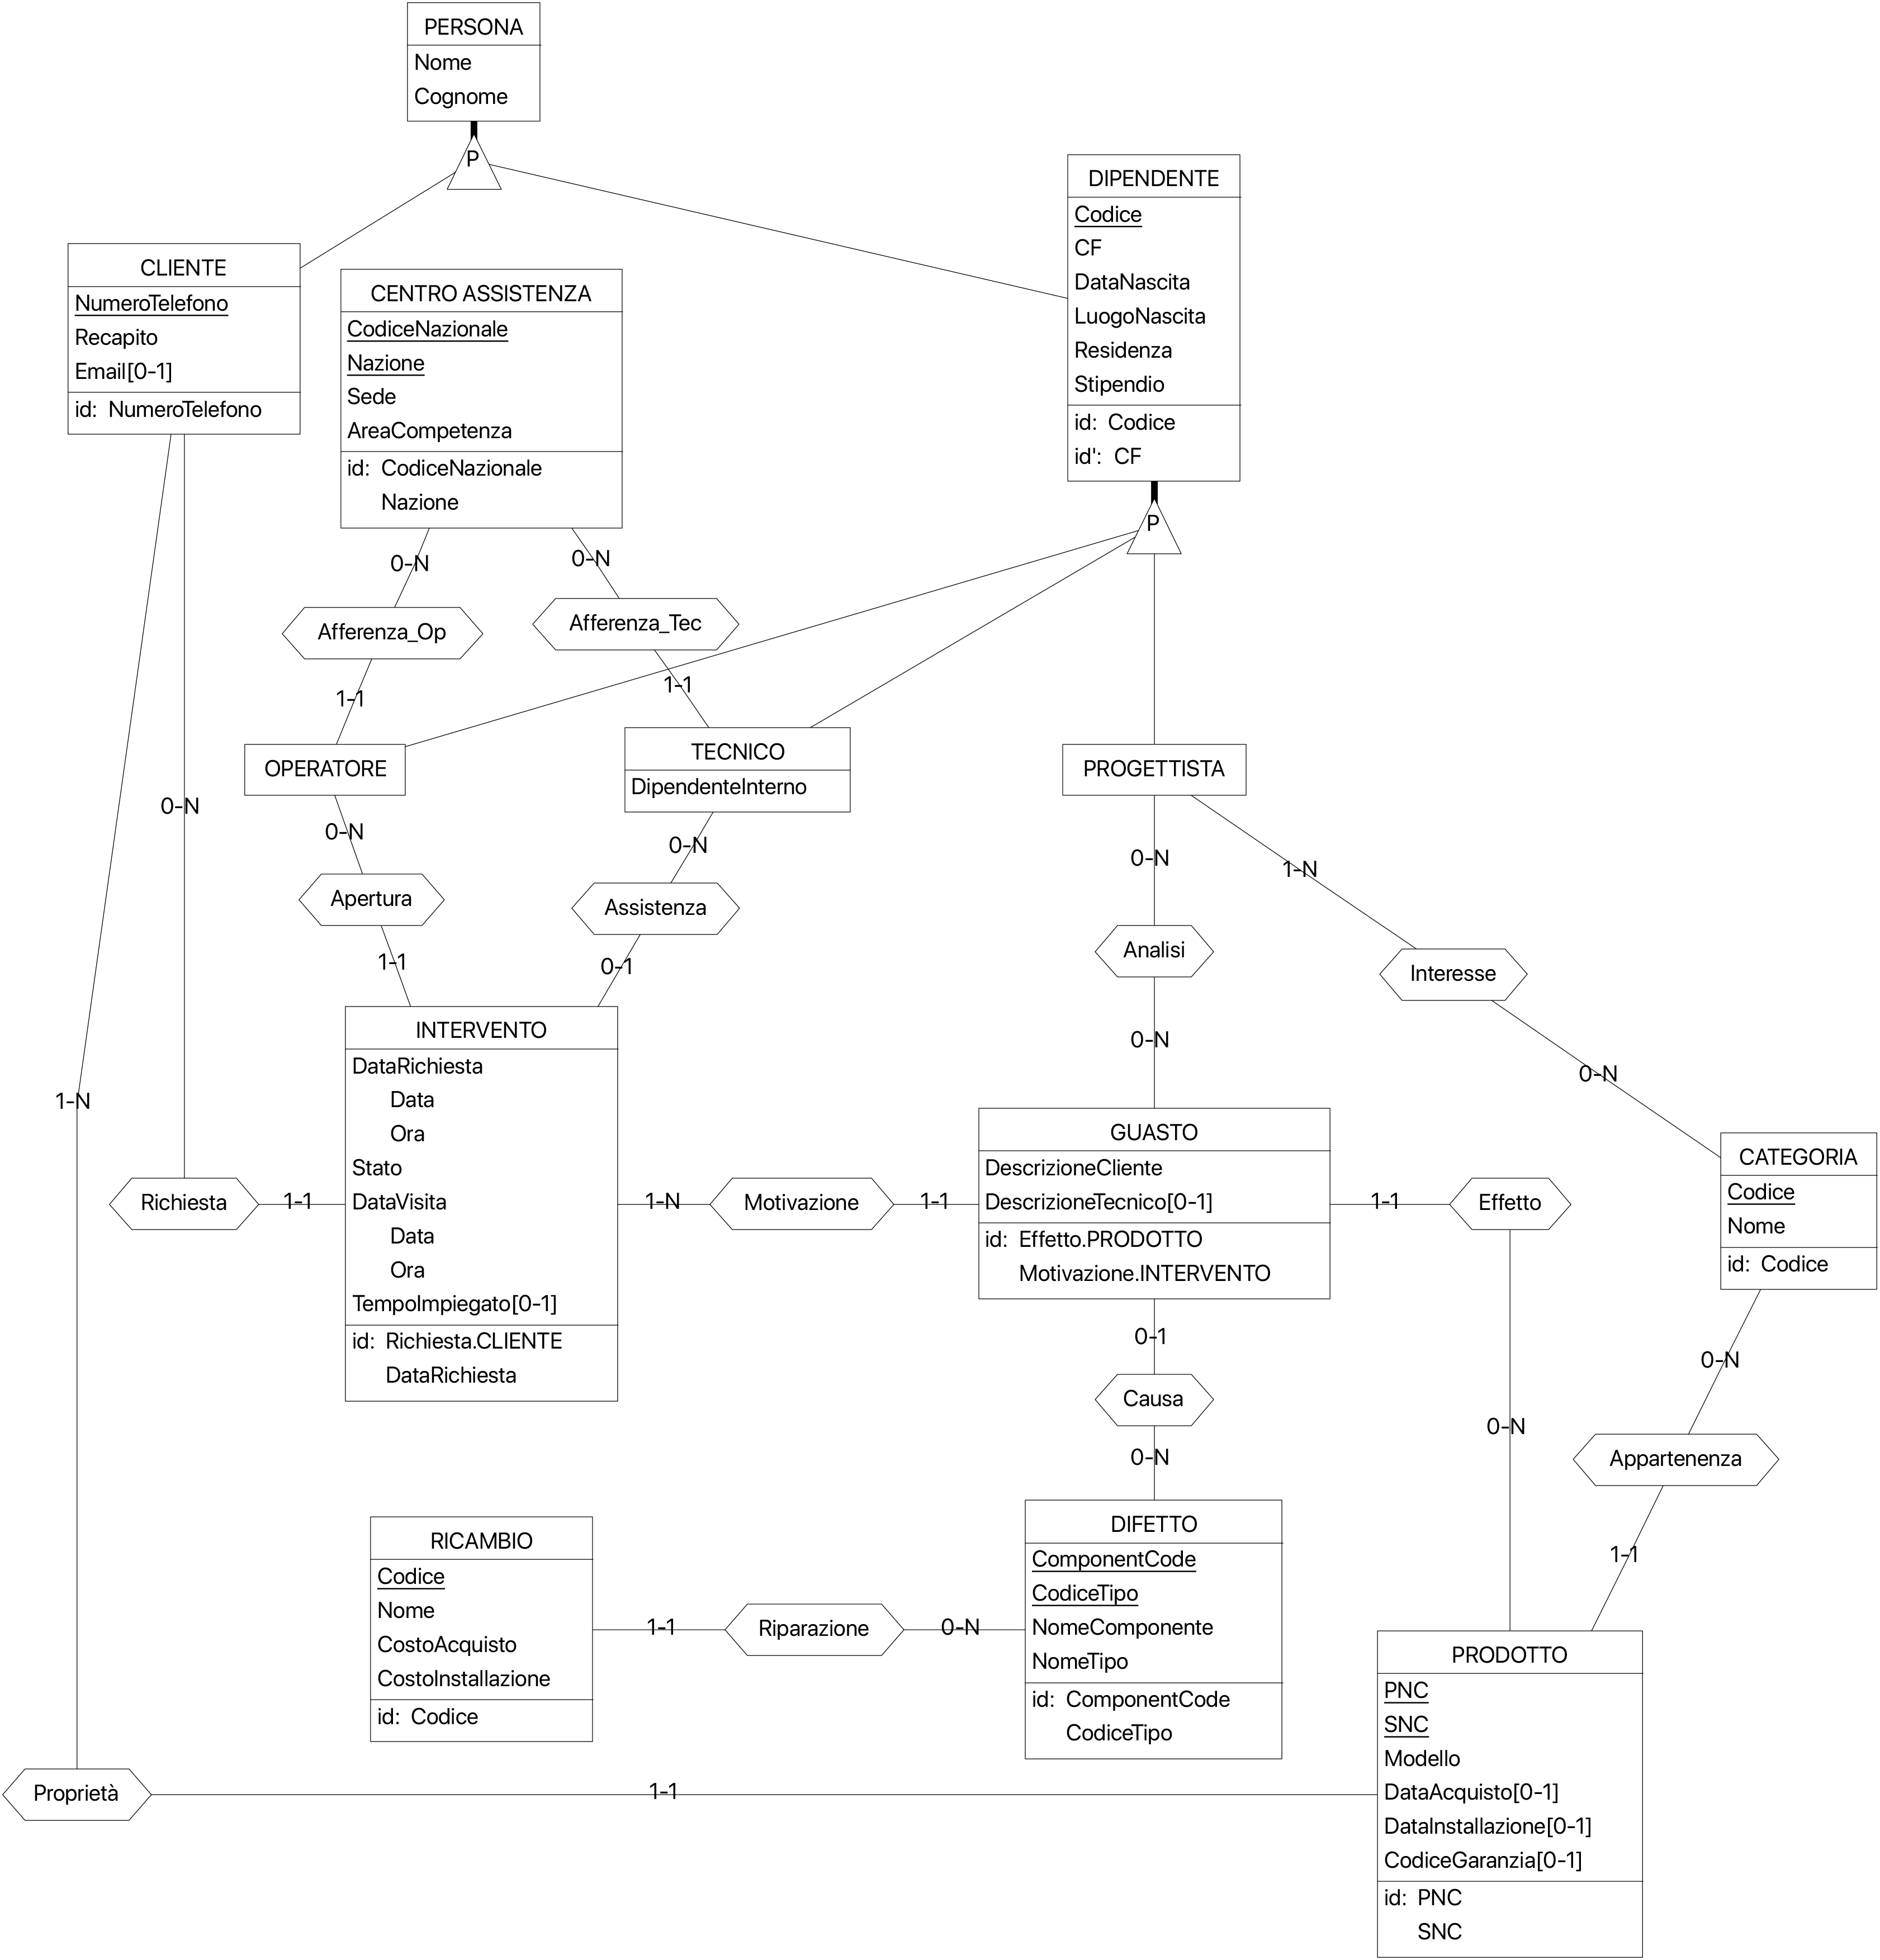
\includegraphics[width=\linewidth]{images/conceptual.png}
	\caption{Schema concettuale finale}
\end{figure}

I vincoli che questo schema non può modellare sono chiaramente quelli inerenti allo stato delle entità nel tempo, non è infatti lo schema adatto per poter
specificare chi e come dovrà modificare lo stato dell'intervento una volta creatone uno nuovo. Inoltre, non è possibile specificare nello schema che i guasti
di cui un progettista deve occuparsi sono solamente quelli che riguardano prodotti appartenenti alla sua categoria di interesse. 

\chapter{Progettazione logica}

\section{Volume dei dati}

\begin{tabularx}{\linewidth}{>{\hsize=0.375\hsize}X|X|>{\hsize=0.475\hsize}X}
	\hline
	\textbf{Nome del concetto} & \textbf{Tipo di costrutto} & \textbf{Stima del volume}\\
	\hline
	\hline
	Persona & E & 13.350\\
	\hline
	Dipendente & E & 450\\
	\hline
	Cliente & E & 12.900\\
	\hline
	Operatore & E & 80\\
	\hline
	Tecnico & E & 240\\
	\hline
	Progettista & E & 130\\
	\hline
	Centro Assistenza & E & 80\\
	\hline
	Afferenza\_Tec & R & 240\\
	\hline
	Afferenza\_Op & R & 80\\
	\hline
	Intervento & E & 13.200\\
	\hline
	Richiesta & R & 13.200\\
	\hline
	Apertura & R & 13.200\\
	\hline
	Assistenza & R & 13.200\\
	\hline
	Motivazione & R & 13.220\\
	\hline
	Guasto & E & 13.220\\
	\hline
	Analisi & R & 429.650\\
	\hline
	Difetto & E & 50\\
	\hline
	Causa & R & 13.220\\
	\hline
	Ricambio & E & 75\\
	\hline
	Riparazione & R & 75\\
	\hline
	Prodotto & E & 13.000\\
	\hline
	Effetto & R & 13.220\\
	\hline
	Modello & E & 800\\
	\hline
	Tipo & R & 13.000\\
	\hline
	Proprietà & R & 13.000\\
	\hline
	\caption{Tabella dei volumi dei dati}
\end{tabularx}

Questa tabella prende in considerazione i volumi dei dati stimati nell'arco di un anno, immaginando che ogni mese solamente i dati inerenti ai guasti
degli undici mesi precedenti vengano mantenuti, mentre i dati vecchi di un anno o più vengano mantenuti ma solo in modo riassuntivo. In questo modo
possiamo assumere che i volumi dei dati indicati restino all'incirca costanti nel tempo.

\section{Descrizione e frequenza delle principali operazioni}

Le principali operazioni che possono essere fatti sulla base di dati possono essere divise in tre categorie, a seconda del dipendente
dell'azienda che interessano. Se prendiamo in considerazione un operatore, le operazioni più frequenti che deve eseguire sono:

\begin{itemize}
	\item[\textbf{O1} -] Inserimento di un nuovo intervento
		\subitem Un operatore dovrà poter inserire un nuovo intervento 
	\item[\textbf{O2} -] Cancellazione di un intervento precedentemente aperto dall'operatore
		\subitem Un operatore dovrà poter cancellare un intervento aperto in precedenza da lui stesso perché accortosi di un errore commesso nell'inserimento
		oppure perché il cliente non desidera più ricevere alcun tipo di assistenza
\end{itemize}

Se consideriamo invece un tecnico, le operazioni più frequenti che riguardano l'esecuzione delle sue mansioni sono:

\begin{itemize}
	\item[\textbf{T1 -}] Vista di tutti gli interventi correntemente aperti non già assegnati ad un altro tecnico, ordinati per urgenza
		\subitem Prima di iniziare a lavorare, un tecnico dovrà capire quali sono gli interventi sui quali potrà dedicarsi e per poter scegliere, deve poterli avere a
		disposizione tutti quanti. In particolar modo, sarebbe più utile organizzarli per urgenza, qui intesa come tempo trascorso dalla data della chiamata
	\item[\textbf{T2 -}] Aggiornamento di un intervento
		\subitem Una volta recatosi a casa di un cliente, il tecnico avrà avuto la possibilità di aggiungere al sistema le informazioni sul prodotto che il cliente
		non era riuscito a fornire. Inoltre, dopo aver eseguito la riparazione, sarà necessario che aggiunga anche le informazioni sull'intervento di sua sola competenza
\end{itemize}

Da ultimo, ci sono i progettisti che necessiteranno di stilare rapporti sotto forma di classifiche sulle principali caratteristiche dei guasti. Le principali operazioni che
permettono di estrarre dati di loro interesse sono:

\begin{itemize}
	\item[\textbf{P1 -}] Visualizzare tutti i guasti accaduti nel mese corrente
		\subitem Ogni mese è richiesto fare un \textit{report} sulla produzione degli elettrodomestici ed è perciò necessario avere a disposizione tutti i guasti che sono accaduti in questo periodo
	\item[\textbf{P2 -}] I primi cinque modelli che hanno subito più guasti nel mese corrente
		\subitem Di tutti i guasti, quelli più importanti saranno quelli che coinvolgono i modelli maggiormente colpiti, gli stessi che necessiteranno uno studio più approfondito per analizzarne 
		le criticità
	\item[\textbf{P3 -}] I primi cinque \textit{PNC} che hanno subito più guasti nel mese corrente
		\subitem Ogni modello coinvolge più codici di prodotto e per un'analisi di in maggior dettaglio è necessario poter avere a disposizione una classifica
		di guasti ordinata per \textit{PNC}, da cui estrarre i più colpiti
	\item[\textbf{P4 -}] I primi cinque \textit{Component Code} che sono stati coinvolti maggiormente nei guasti di questo mese
		\subitem Alcuni componenti si guastano più di altri indipendentemente dal prodotto sul quale sono collocati. Si vuole ottenere i primi cinque maggiormente presenti nei guasti di questo 
		mese
	\item[\textbf{P5 -}] I primi cinque ricambi più utilizzati per riparare i guasti di questo mese
		\subitem Uno stesso ricambio può essere utilizzato in riparazioni di diversi guasti. Quelli più notevoli saranno quelli il cui costo è quello che andrà ad incidere maggiormente su quello 
		totale dei ricambi acquistati per le riparazioni, quindi quelli utilizzati in maggior numero. Si rende perciò necessario stilare una classifica dei ricambi più utilizzati nei guasti del 
		mese corrente
	\item[\textbf{P6 -}] I primi cinque interventi più costosi a partire dai ricambi nel mese corrente
		\subitem Il costo di un intervento è principalmente determinato dal costo dei ricambi utilizzati nella sua riparazione, è perciò interessante
		determinare per l'analisi dei costi i cinque interventi più costosi del mese in termini di ricambi impiegati
	\item[\textbf{P7 -}] I primi cinque paesi per numero di guasti avvenuti in questo mese
		\subitem Per dare una "localizzazione spaziale" ai guasti, cioè individuare quali paesi hanno gli stabilimenti produttivi con un tasso di difettosità più alto, è bene
		poter classificare i vari paesi sulla base del numero di guasti riparati dai centri assistenza che si trovano sul territorio del paese stesso nel mese corrente.
	\item[\textbf{P8 -}] I \textit{Time To Failure} rispetto alla data di acquisto di ciascun prodotto coinvolto nei guasti di questo mese
		\subitem Un altro indicatore spesso utilizzato nell'elaborazione dei guasti è il cosiddetto "\textit{Time To Failure}", cioè il tempo impiegato da un particolare elettrodomestico
		per subire un guasto. In questo caso è calcolato a partire dal momento in cui l'elettrodomestico è stato acquistato.
	\item[\textbf{P9 -}] I \textit{Time To Failure} rispetto alla data di installazione di ciascun prodotto coinvolto nei guasti di questo mese
		\subitem Come l'operazione precedente, solamente che il \textit{Time To Failure} è calcolato a partire dalla data di installazione del prodotto.
	\item[\textbf{P10 -}] Tempo medio di riparazione di un guasto per tipo di difetto
		\subitem Una distinzione per costo tra i guasti può essere fatta anche nei termini del tempo medio di riparazione dei guasti associati ad un particolare tipo di difetto,
		andando ad indicare su quali parti di ciascun prodotto è necessario focalizzarsi per ridurre i costi di manutenzione dei prodotti stessi
\end{itemize}

Le operazioni che non vanno eseguite da una specifica categoria di dipendenti, ma riguardano più delle informazioni utili all'azienda in generale, sono:

\begin{itemize}
	\item[\textbf{V1} -] Conteggio di tutti gli interventi aperti nel mese da ciascun operatore
		\subitem Per valutare l'efficienza e la preparazione degli operatori dei centri assistenza, nonché pagare gli stipendi a ciascun operatore, deve essere
		possibile visualizzare il conteggio degli interventi aperti nel mese corrente da ciascun operatore
	\item[\textbf{V2 -}] Conteggio di tutti gli interventi chiusi nel mese corrente da ciascun tecnico
		\subitem Per valutare l'efficienza e la preparazione dei tecnici dei centri assistenza, nonché per poter pagare gli stipendi, deve essere
		possibile visualizzare il conteggio degli interventi chiusi nel mese corrente da ciascun operatore
	\item[\textbf{V3 -}] Tempo medio di riparazione di un guasto per ciascun tecnico
		\subitem Altro parametro di interesse nell'analisi dell'efficienza e della preparazione di un tecnico è il tempo impiegato in media per riparare i guasti
		che decide di voler sottoporre alla sua attenzione
	\item[\textbf{V4 -}] Distanza temporale media tra ricezione della chiamata e visita del tecnico per centro assistenza
		\subitem La "bontà" di un centro assistenza si può valutare sulla base di quanto rapidamente riesce a risolvere i vari interventi sottoposti. Si rende perciò
		utile poter calcolare per ogni centro assistenza la velocità media di risoluzione degli interventi.
\end{itemize}

\begin{tabularx}{\linewidth}{X|X|X}
	\hline
	\textbf{Codice operazione} & \textbf{Frequenza} & \textbf{Tipo (Interattiva / Batch)}\\
	\hline
	\hline
	O1 & 5 volte al giorno & I\\
	\hline
	O2 & 1 volta al mese & I\\
	\hline
	T1 & 1 volta al giorno & I\\
	\hline
	T2 & 5 volte al giorno & I\\
	\hline
	P1 & 5 volte al mese & B\\
	\hline
	P2 & 5 volte al mese & B\\
	\hline
	P3 & 5 volte al mese & B\\
	\hline
	P4 & 5 volte al mese & B\\
	\hline
	P5 & 5 volte al mese & B\\
	\hline
	P6 & 5 volte al mese & B\\
	\hline
	P7 & 5 volte al mese & B\\
	\hline
	P8 & 2 volte al mese & B\\
	\hline
	P9 & 2 volte al mese & B\\
	\hline
	P10 & 2 volte al mese & B\\
	\hline
	V1 & 1 volta al mese & B\\
	\hline
	V2 & 1 volta al mese & B\\
	\hline
	V3 & 1 volta al mese & B\\
	\hline
	V4 & 1 volta al mese & B\\
	\hline
	\caption{Tabella della frequenza delle principali operazioni}
\end{tabularx}

Nella precedente tabella vengono riassunte le frequenze e i tipi di tutte le operazioni che sono state individuate.

\section{Schemi di navigazione e tabelle degli accessi delle principali operazioni}

Per ogni operazione, verrà esplicitato a parole il modo con il quale verrà eseguita l'operazione e verrà mostrato uno schema che indichi come questi
accessi alle varie entità e relazioni si riflette sullo schema concettuale realizzato. Da questo schema, si estrarrà la tabella degli accessi che ci
permetterà di avere il costo totale di ognuna delle operazioni in termini di "\textit{I/O}".

\subsection{O1, O2 - Inserimento e cancellazione di un nuovo intervento}

L'apertura di ogni nuovo intervento coinciderà con l'aggiunta di un nuovo intervento e, nel caso peggiore, anche di un nuovo cliente che non aveva mai chiamato
prima d'ora e di uno o più nuovi prodotti che non si erano mai rotti. All'intervento viene inoltre associato l'operatore che lo registra.\newline
L'operazione di cancellazione è identica nelle operazioni, ne cambia semplicemente la frequenza.

\begin{figure}[H]
	\centering
	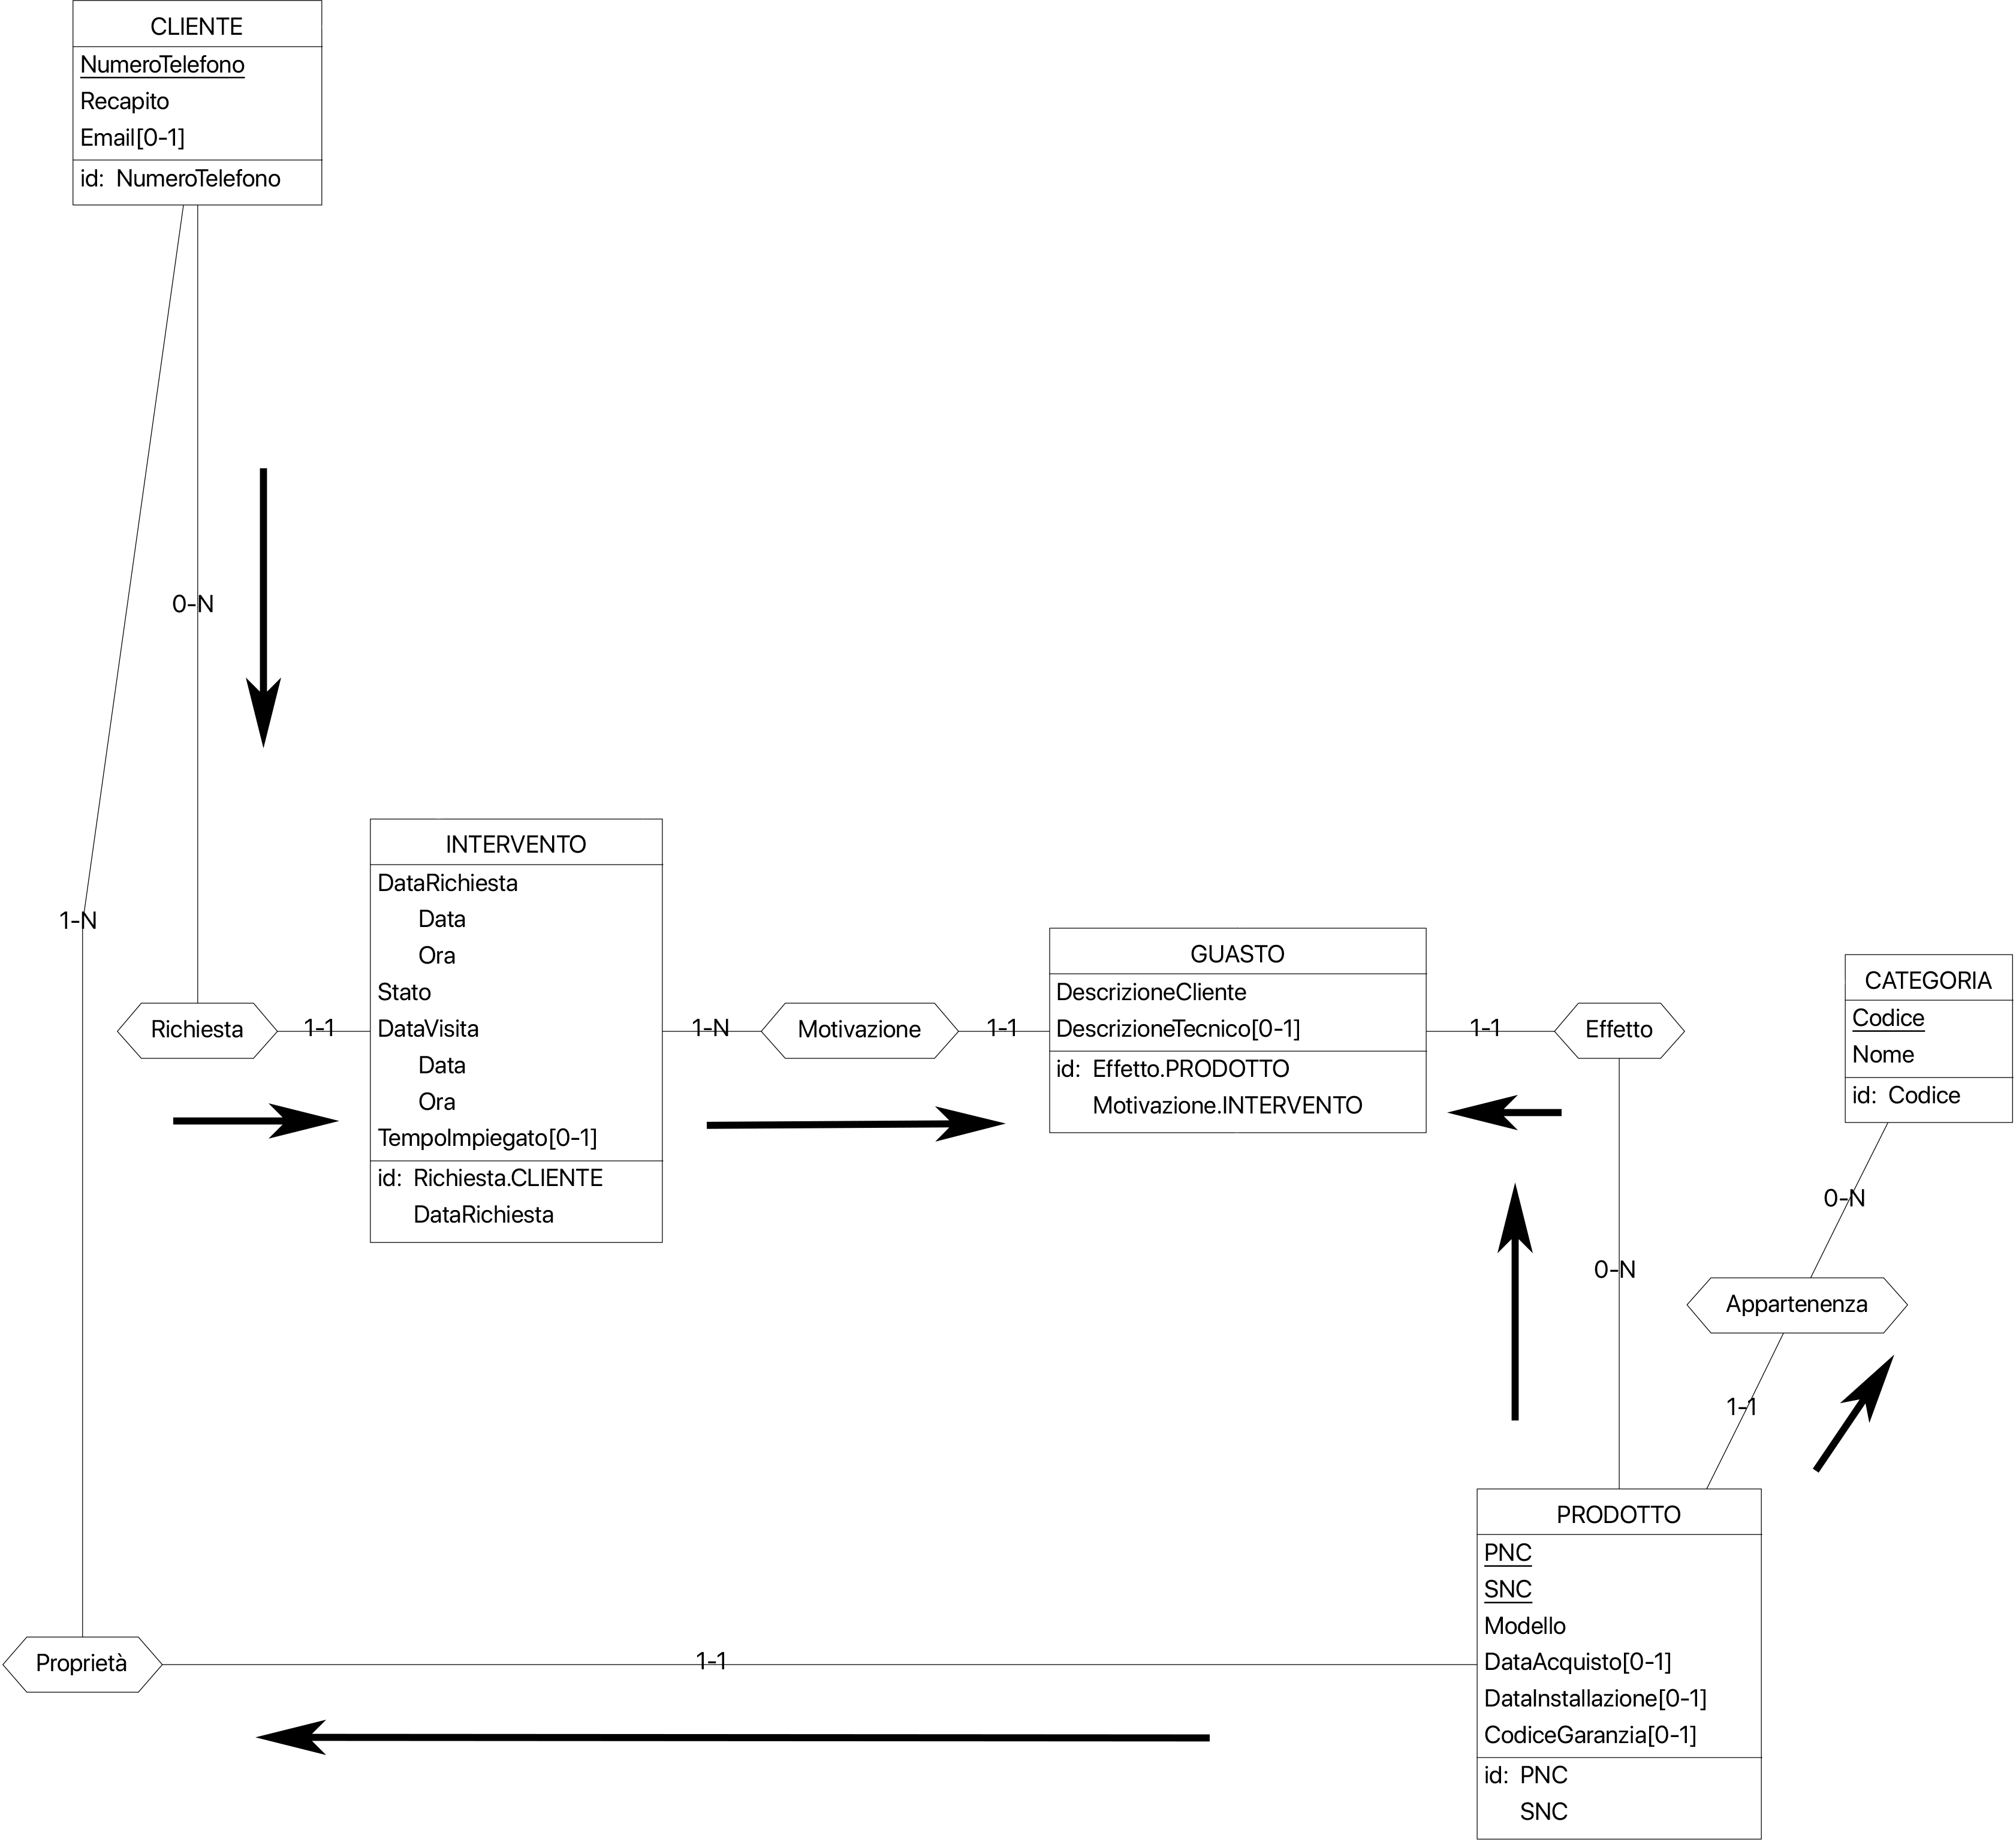
\includegraphics[width=\linewidth]{images/O1-O2.png}
	\caption{Schema di navigazione per le operazioni O1 e O2}
\end{figure}

\begin{tabularx}{\linewidth}{X|X|X}
	\hline
	\textbf{Costrutto coinvolto} & \textbf{Accessi} & \textbf{Tipo di Accesso}\\
	\hline
	\hline
	Intervento & 1 & S\\
	\hline
	Cliente & 1 & S\\
	\hline
	Guasto & 13.220 / 13.200 = 1,002 & S\\
	\hline
	Prodotto & 13.220 / 13.200 = 1,002 & S\\
	\hline
	\hline
	TOTALE & \multicolumn{2}{>{\hsize=2\hsize}X}{ 8,008 Accessi }\\\hline
	\hline
	\caption{Calcolo degli accessi delle operazioni O1 e O2}
\end{tabularx}

\subsection{T1 - Visualizzazione degli interventi aperti}

Questa operazione visualizza tutti e soli gli interventi correntemente aperti, perciò i costrutti che coinvolge sono banali:
solamente l'entità intervento.

\begin{figure}[H]
	\centering
	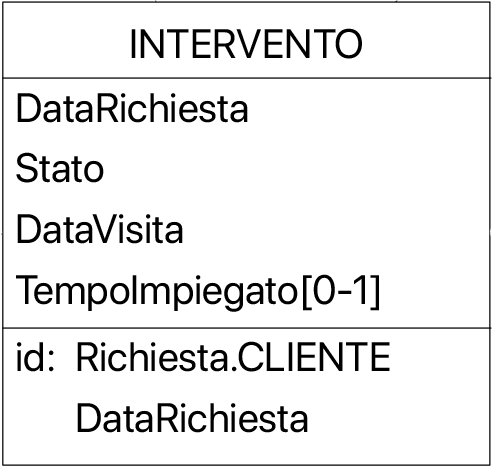
\includegraphics[width=\linewidth]{images/T1.png}
	\caption{Schema di navigazione per l'operazione T1}
\end{figure}

\begin{tabularx}{\linewidth}{X|X|X}
	\hline
	\textbf{Costrutto coinvolto} & \textbf{Accessi} & \textbf{Tipo di Accesso}\\
	\hline
	\hline
	Intervento & 13.200 & L\\
	\hline
	\hline
	TOTALE & \multicolumn{2}{>{\hsize=2\hsize}X}{ 13.200 Accessi }\\\hline
	\hline
	\caption{Calcolo degli accessi dell'operazione T1}
\end{tabularx}

\subsection{T2 - Chiusura di un intervento}

Si tratta di un'operazione svolta da un tecnico una volta giunto a casa di un cliente fatta dopo la riparazione dell'elettrodomestico del cliente. I dati necessariamente
aggiornati sono quelli relativi all'intervento e a ciascuno dei guasti riparati mentre quelli che potrebbero essere inseriti in aggiunta nel caso peggiore sono quelli
relativi al prodotto o ai prodotti che il cliente non è riuscito a reperire da solo.

\begin{figure}[H]
	\centering
	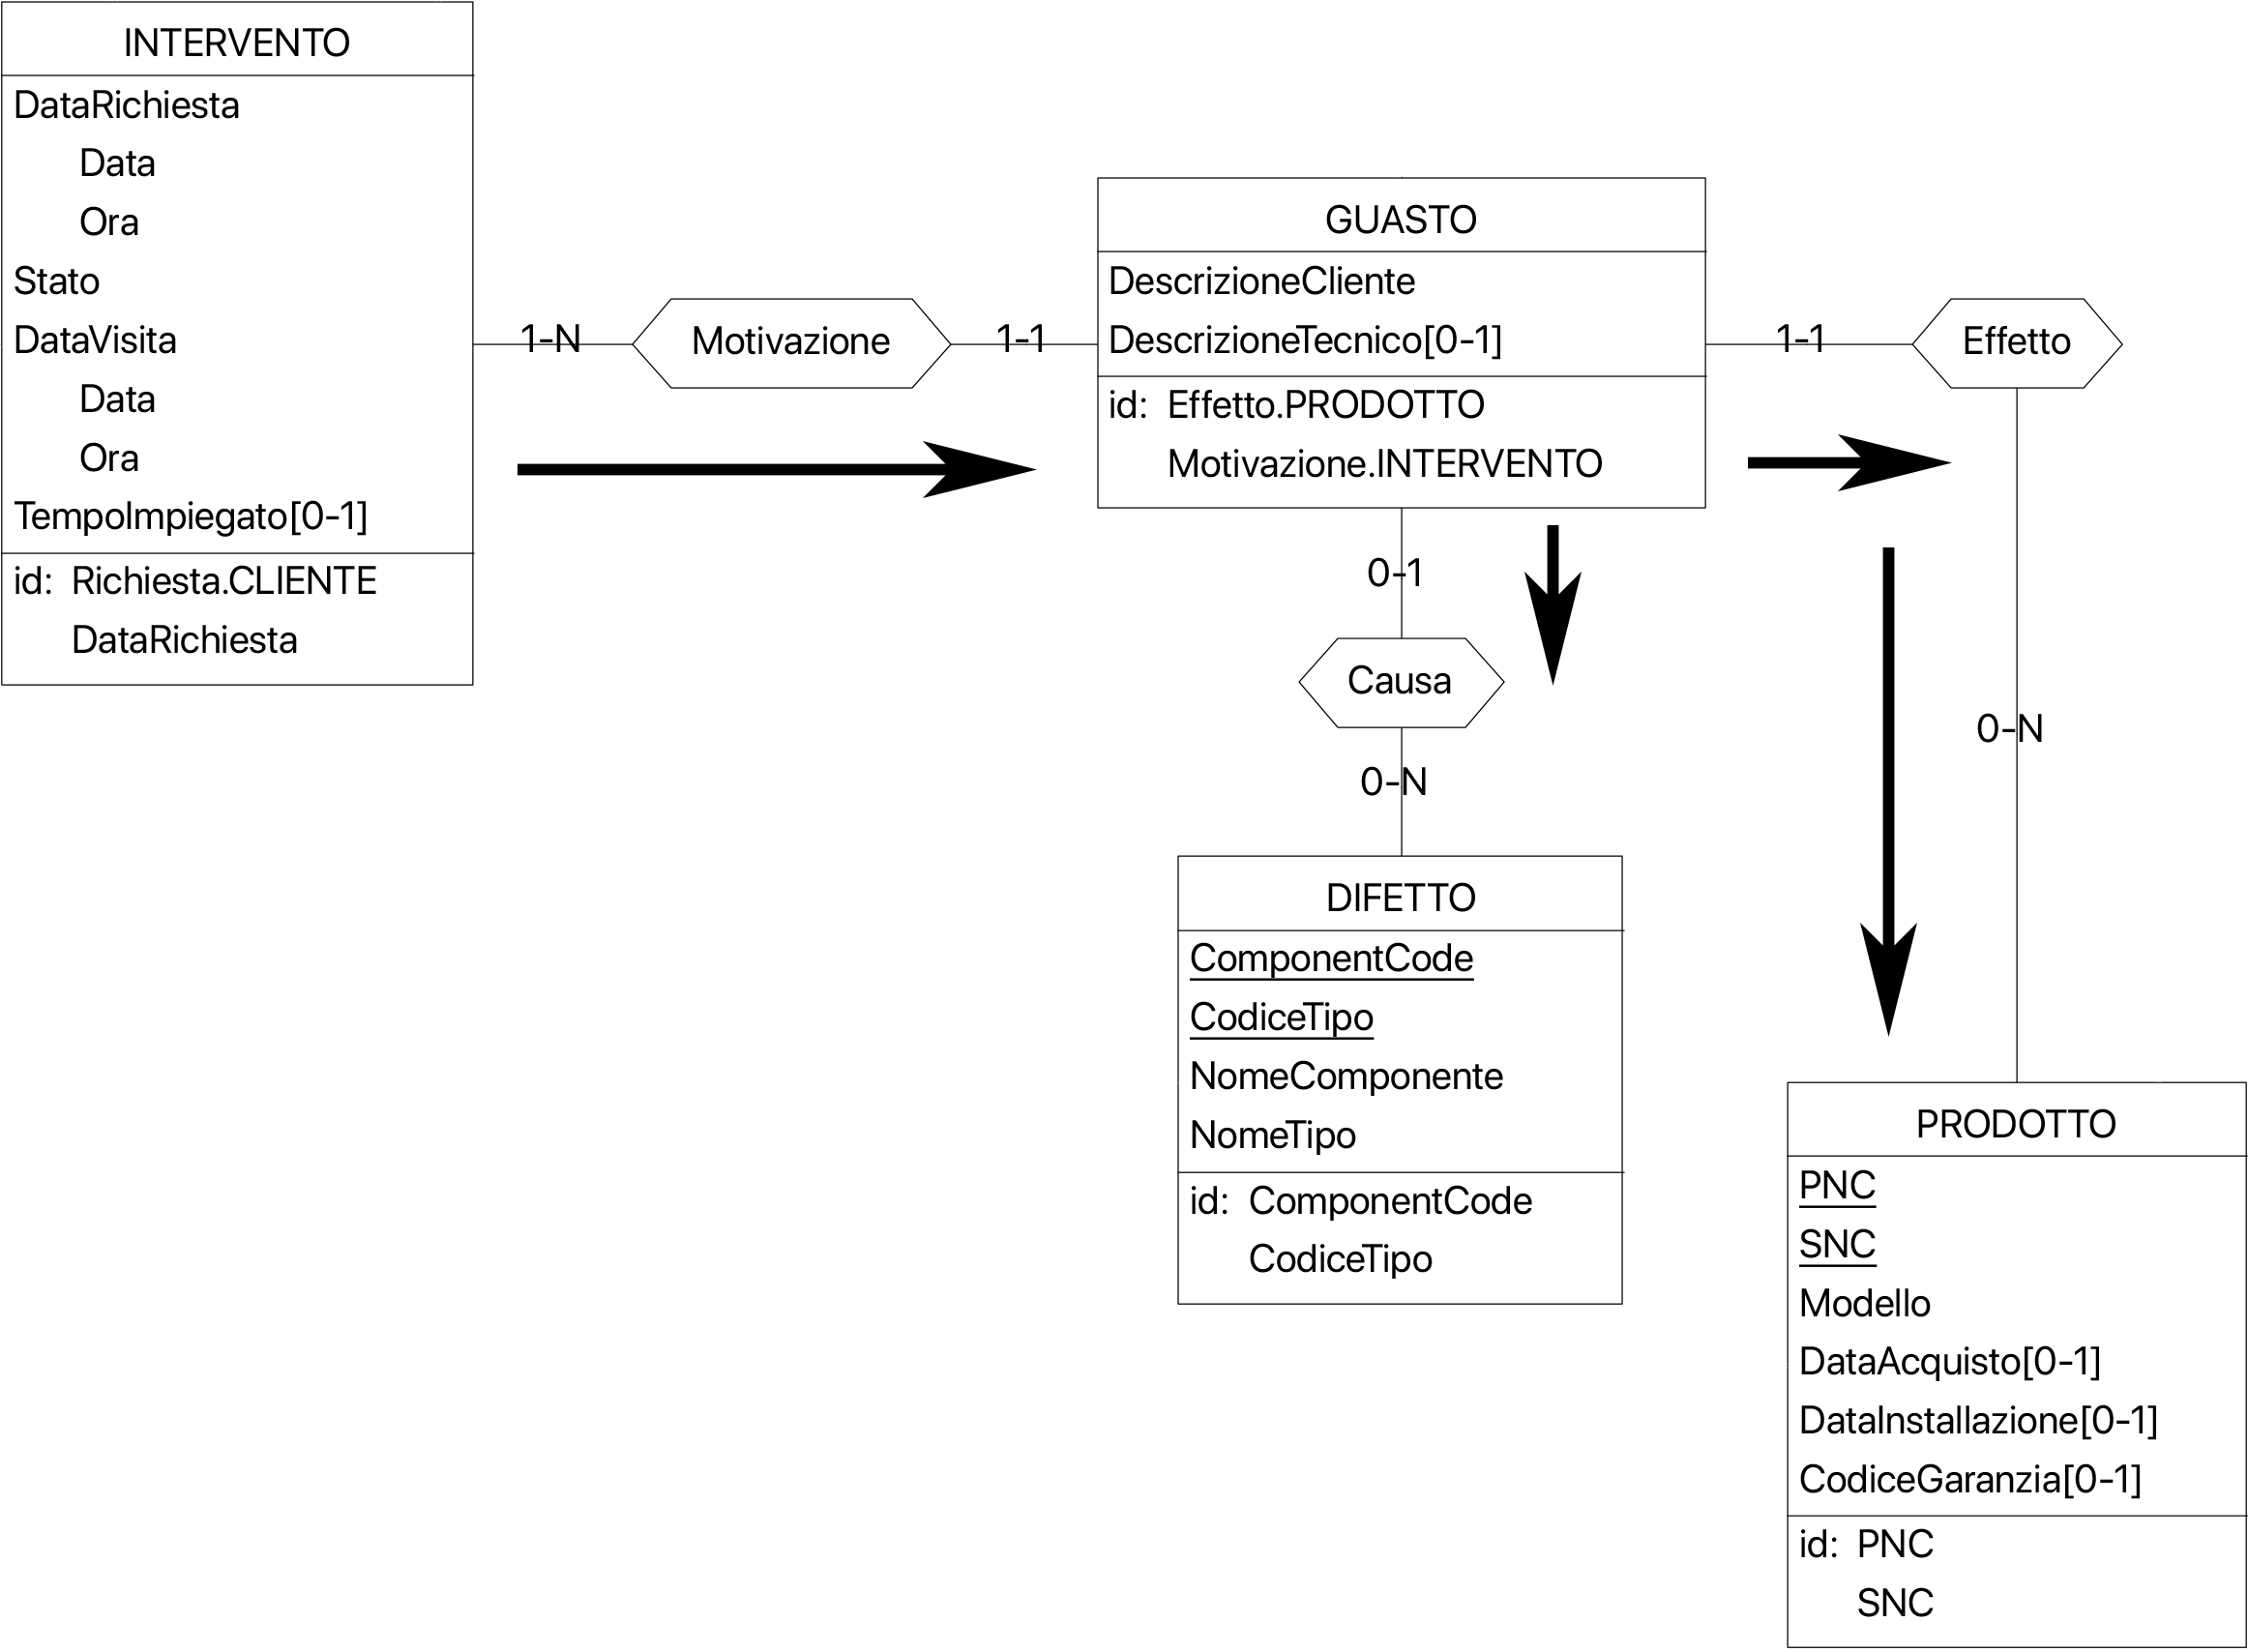
\includegraphics[width=\linewidth]{images/T2.png}
	\caption{Schema di navigazione per l'operazione T2}
\end{figure}

\begin{tabularx}{\linewidth}{X|X|X}
	\hline
	\textbf{Costrutto coinvolto} & \textbf{Accessi} & \textbf{Tipo di Accesso}\\
	\hline
	\hline
	Intervento & 1 & L\\
	\hline
	Intervento & 1 & S\\
	\hline
	Guasto & 13.220 / 13.200 = 1,002 & L\\
	\hline
	Guasto & 13.220 / 13.200 = 1,002 & S\\
	\hline
	Prodotto & 13.220 / 13.200 = 1,002 & L\\
	\hline
	Prodotto & 13.220 / 13.200 = 1,002 & S\\
	\hline
	\hline
	TOTALE & \multicolumn{2}{>{\hsize=2\hsize}X}{ 9,012 Accessi }\\\hline
	\hline
	\caption{Calcolo degli accessi dell'operazione T2}
\end{tabularx}

\subsection{P1 - Visualizzazione di tutti i guasti del mese}

Per visualizzare tutti i guasti accaduti nel mese corrente, occorre passare in rassegna tutti gli elementi dell'entità "Guasto" e vedere la data di apertura dell'intervento
a cui sono associati per vedere se sono del mese corrente oppure no.

\begin{figure}[H]
	\centering
	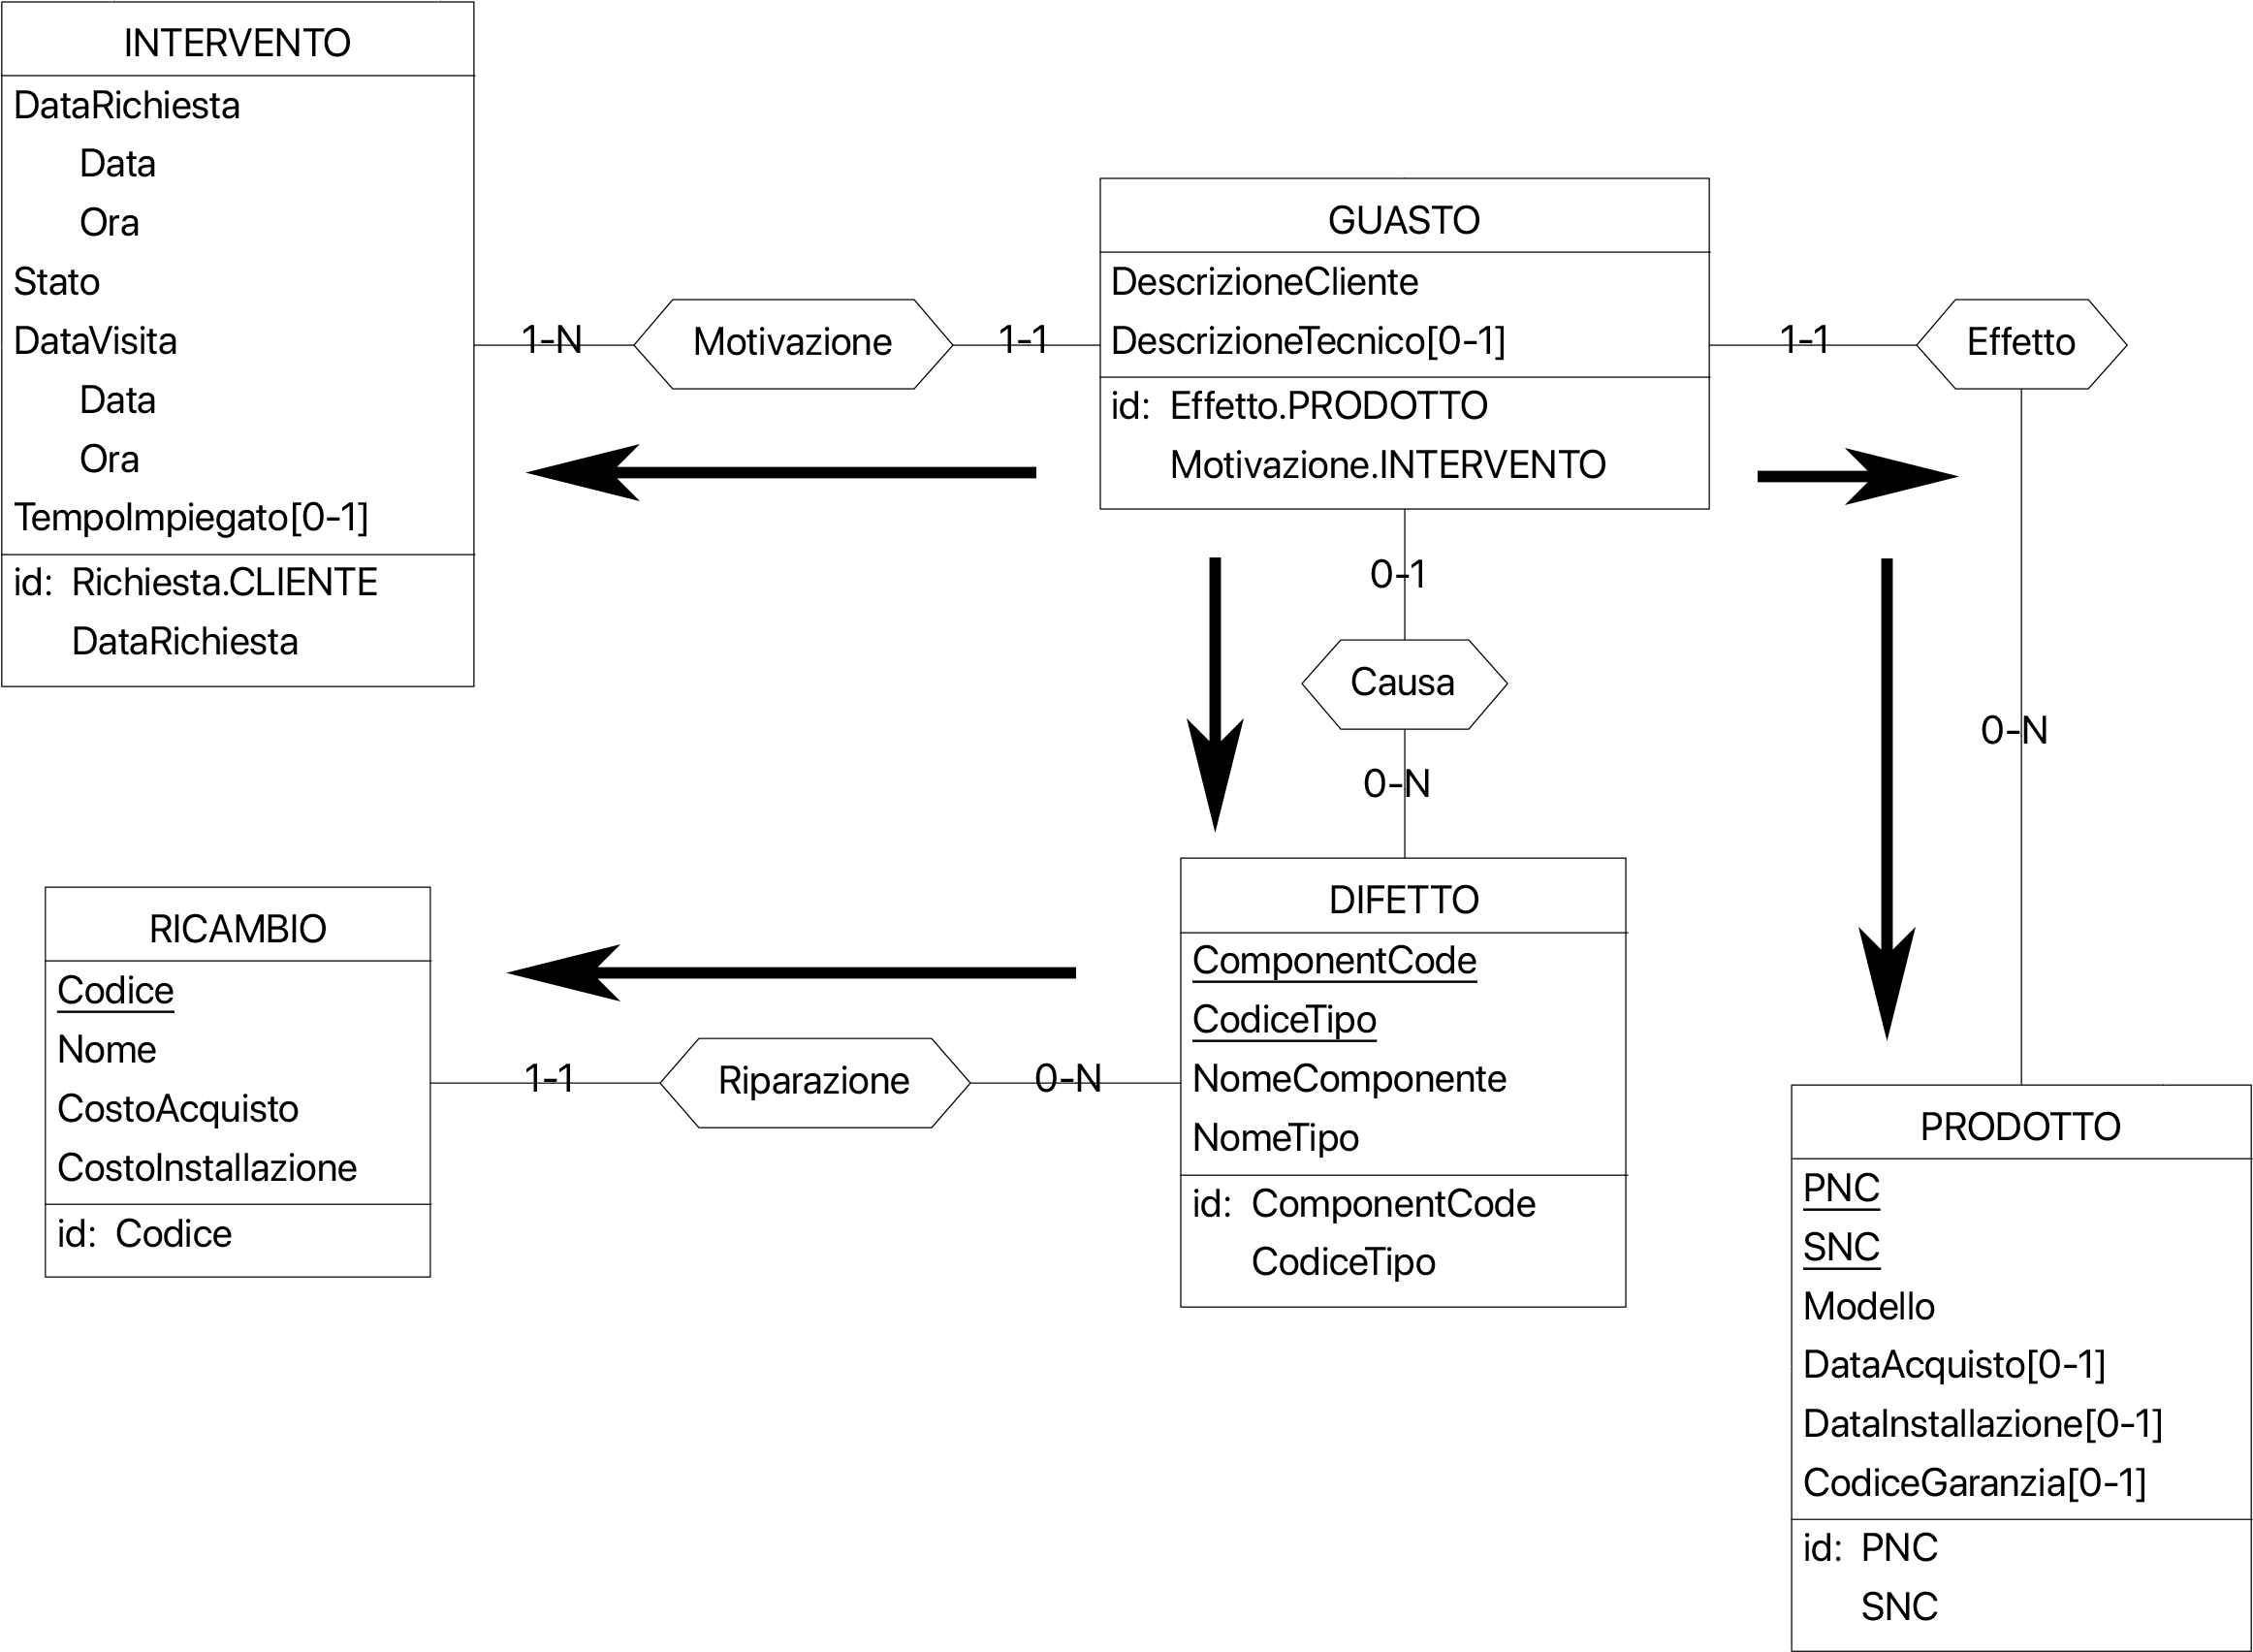
\includegraphics[width=\linewidth]{images/P1.png}
	\caption{Schema di navigazione per l'operazione P1}
\end{figure}

\begin{tabularx}{\linewidth}{X|X|X}
	\hline
	\textbf{Costrutto coinvolto} & \textbf{Accessi} & \textbf{Tipo di Accesso}\\
	\hline
	\hline
	Guasto & 13.220 & L\\
	\hline
	Intervento & 13.220 & L\\
	\hline
	\hline
	TOTALE & \multicolumn{2}{>{\hsize=2\hsize}X}{ 26.440 Accessi }\\\hline
	\hline
	\caption{Calcolo degli accessi dell'operazione P1}
\end{tabularx}

\subsection{P2 - I primi cinque modelli che hanno subito più guasti nel mese corrente}

In questa operazione si considerano i guasti del mese corrente e poi, passando attraverso l'entità "Prodotto", si ottengono i modelli associati a ciascun
guasto, per poi raggrupparli e contare i \textit{record} che compongono ogni gruppo ed infine tenere soltanto i primi cinque. 

\begin{figure}[H]
	\centering
	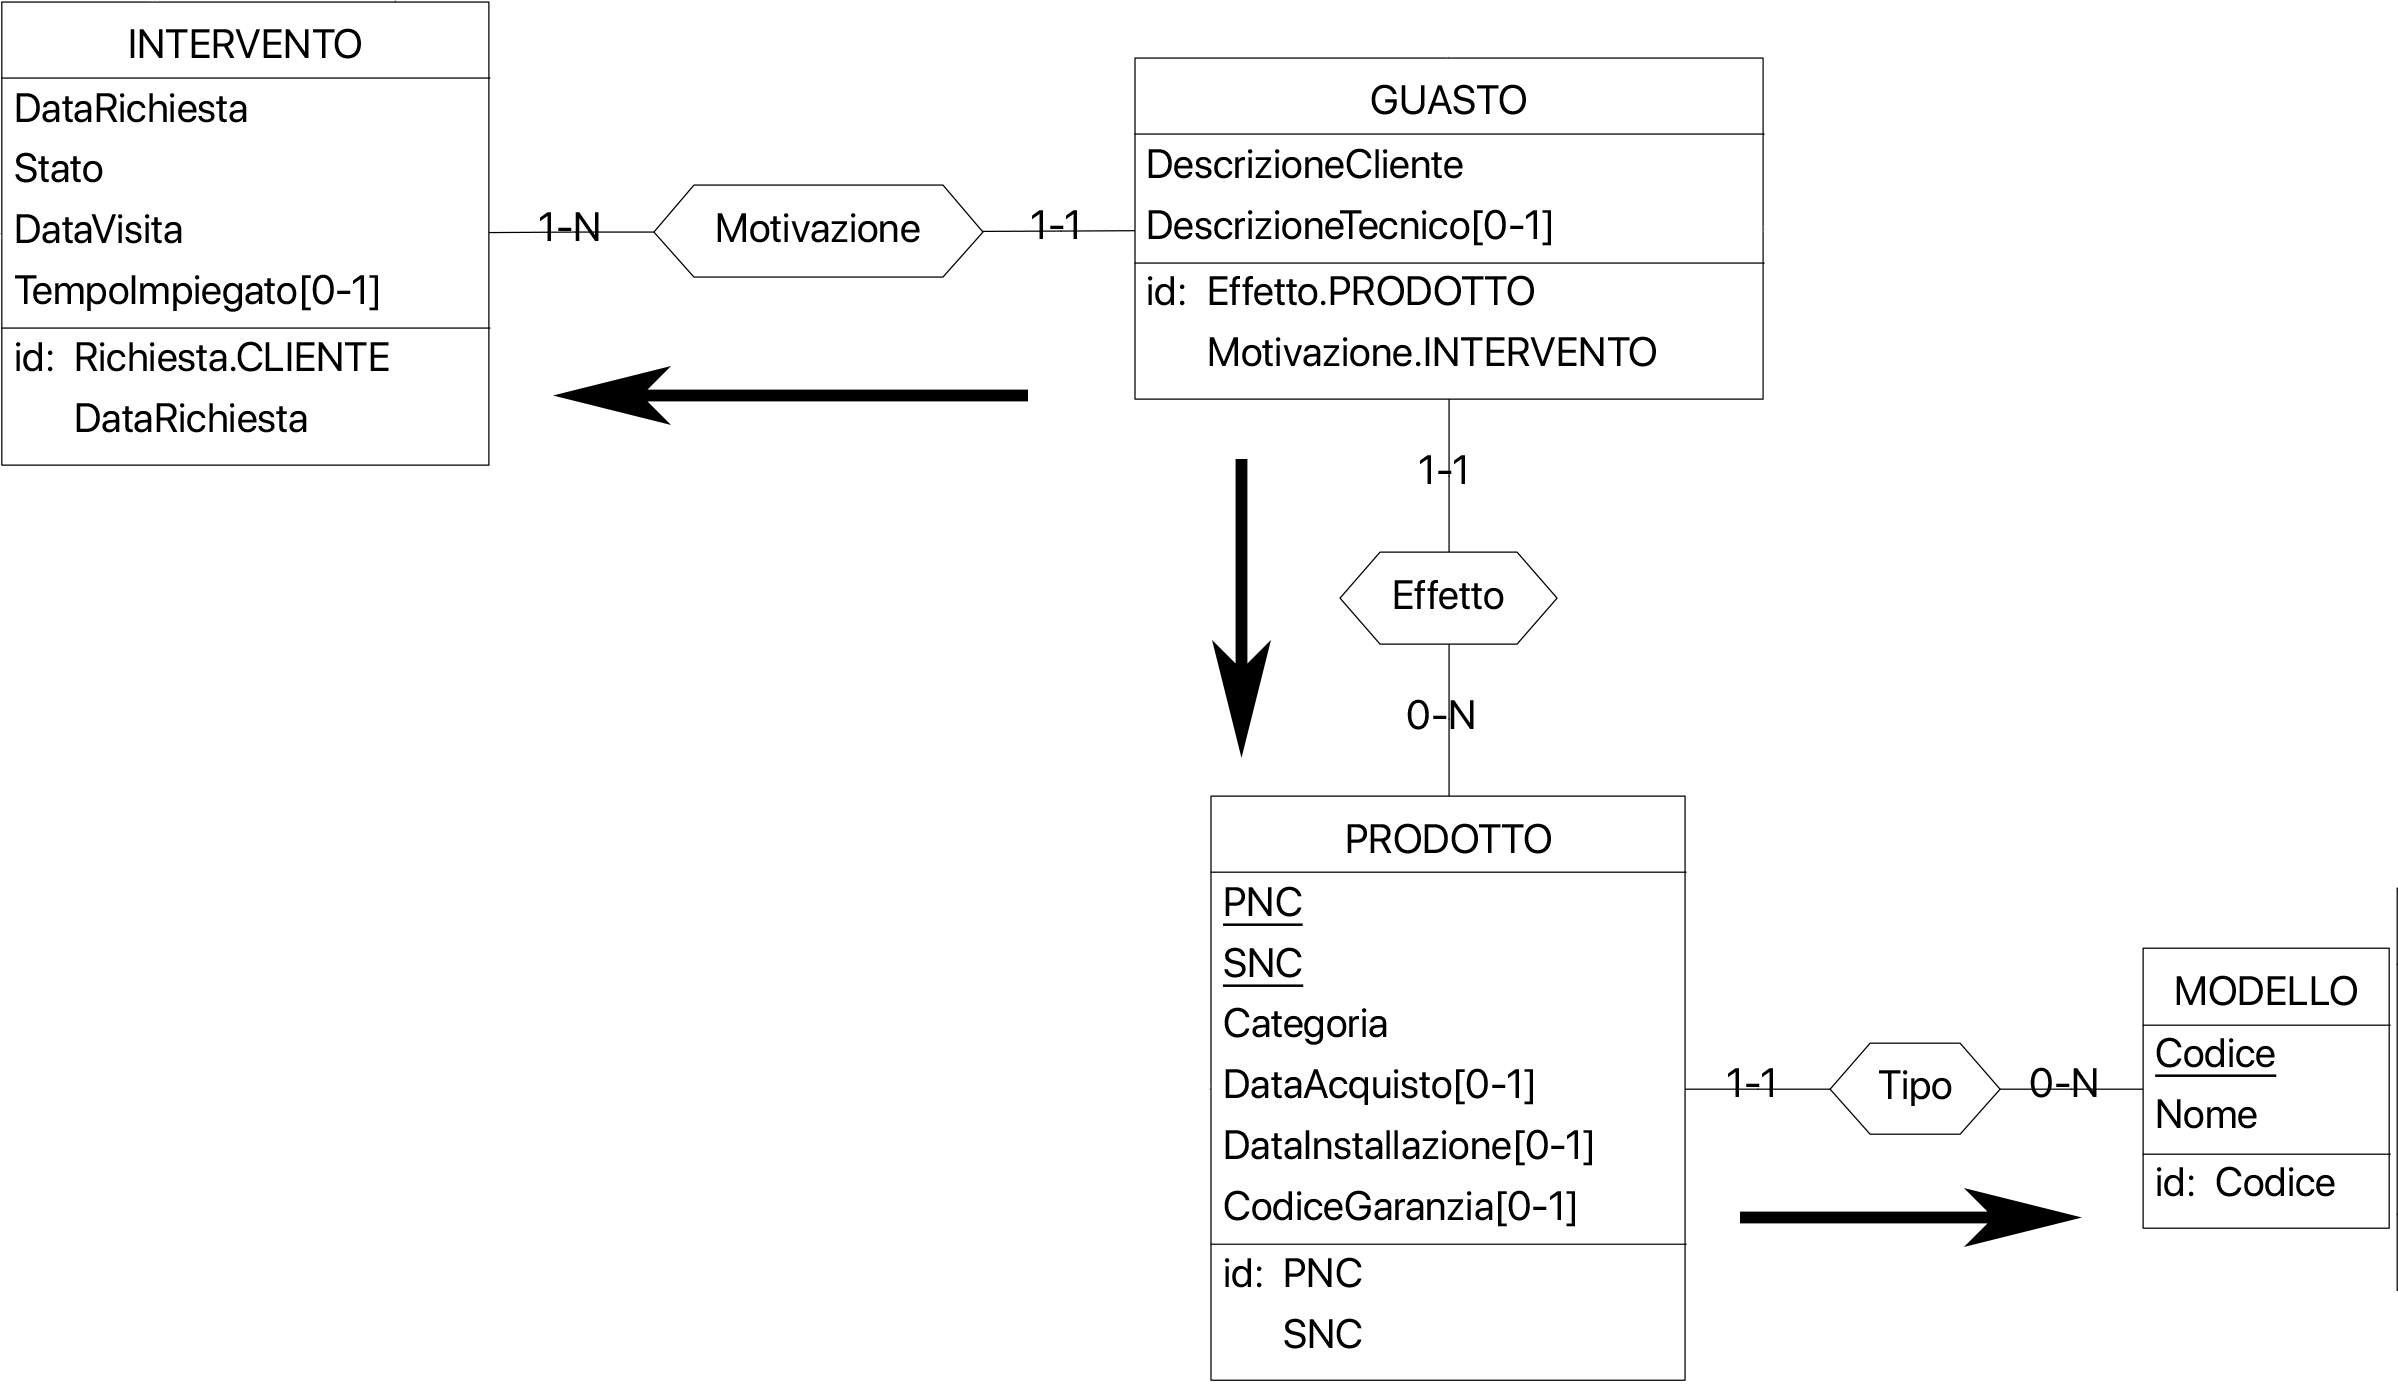
\includegraphics[width=\linewidth]{images/P2.png}
	\caption{Schema di navigazione per l'operazione P2}
\end{figure}

\begin{tabularx}{\linewidth}{X|X|X}
	\hline
	\textbf{Costrutto coinvolto} & \textbf{Accessi} & \textbf{Tipo di Accesso}\\
	\hline
	\hline
	Guasto & 13.220 & L\\
	\hline
	Intervento & 13.220 & L\\
	\hline
	Prodotto & 13.220 / 12 = 1.101,667 & L\\
	\hline
	Modello & 1.101,667 & L\\
	\hline
	\hline
	TOTALE & \multicolumn{2}{>{\hsize=2\hsize}X}{ 28.643,334 Accessi }\\\hline
	\hline
	\caption{Calcolo degli accessi dell'operazione P2}
\end{tabularx}

\subsection{P3, P8, P9 - I primi cinque PNC che hanno subito più guasti e i "Time To Failure" per ciascun prodotto a partire dalla data di acquisto e dalla data di installazione}

L'operazione P3 è pressoché identica alla precedente, con la sola differenza che ci interessa raggruppare per PNC e non per modello, perciò non è necessario andare
a scomodare quest'ultima entità. Per le due operazioni P8 e P9 invece ci si preoccupa di poter estrarre i cosiddetti "Time To Failure" di ciascun prodotto, cioè il
tempo che è passato tra una certa data fissata e il momento in cui il prodotto ha subito il guasto. L'operazione P8 fissa il momento iniziale alla data di acquisto
del prodotto, mentre l'operazione P9 alla data di installazione dello stesso. Anche per queste due operazioni, partendo dai guasti del mese corrente, si risale alla data di apertura
dell'intervento associato, che viene scelta come data di rottura dell'elettrodomestico, e poi si risale al prodotto associato da cui si estrae la data di interesse.

\begin{figure}[H]
	\centering
	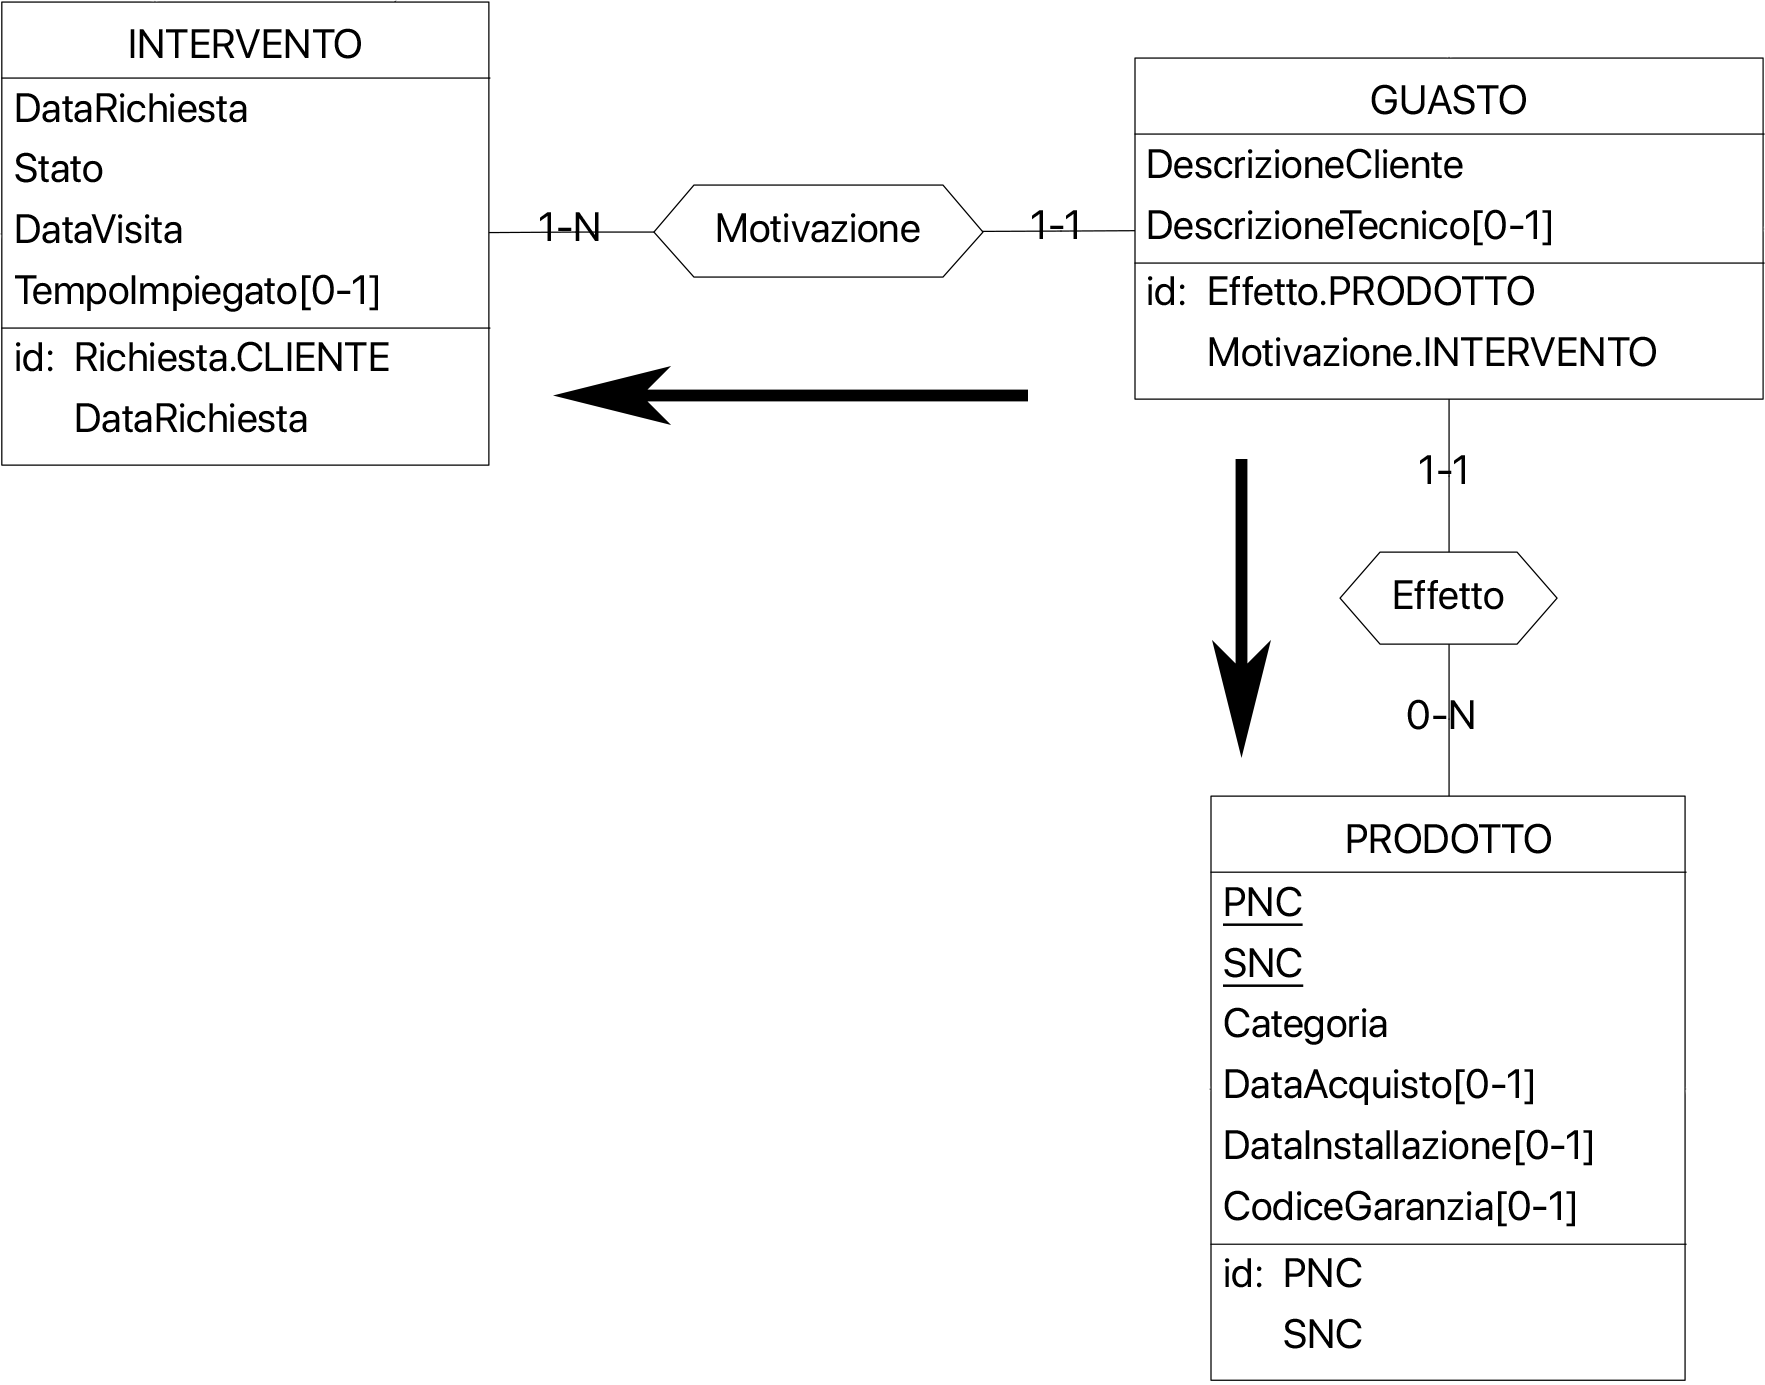
\includegraphics[width=\linewidth]{images/P3-P8-P9.png}
	\caption{Schema di navigazione per l'operazione P3}
\end{figure}

\begin{tabularx}{\linewidth}{X|X|X}
	\hline
	\textbf{Costrutto coinvolto} & \textbf{Accessi} & \textbf{Tipo di Accesso}\\
	\hline
	\hline
	Guasto & 13.220 & L\\
	\hline
	Intervento & 13.220 & L\\
	\hline
	Prodotto & 13.220 / 12 = 1.101,667 & L\\
	\hline
	\hline
	TOTALE & \multicolumn{2}{>{\hsize=2\hsize}X}{ 27.541,667 Accessi }\\\hline
	\hline
	\caption{Calcolo degli accessi dell'operazione P3}
\end{tabularx}

\subsection{P4 - I primi cinque component code maggiormente presenti nei guasti di questo mese}

Anche questa operazione si inserisce sulla scia della precedente, con la differenza che, dopo aver ottenuto tutti i guasti del mese corrente, li si raggruppa sulla base del
\textit{component code} del difetto che li ha causati, per poi contare quanti elementi sono presenti in ogni gruppo e infine ordinare i gruppi sulla base della quantità dei loro membri.

\begin{figure}[H]
	\centering
	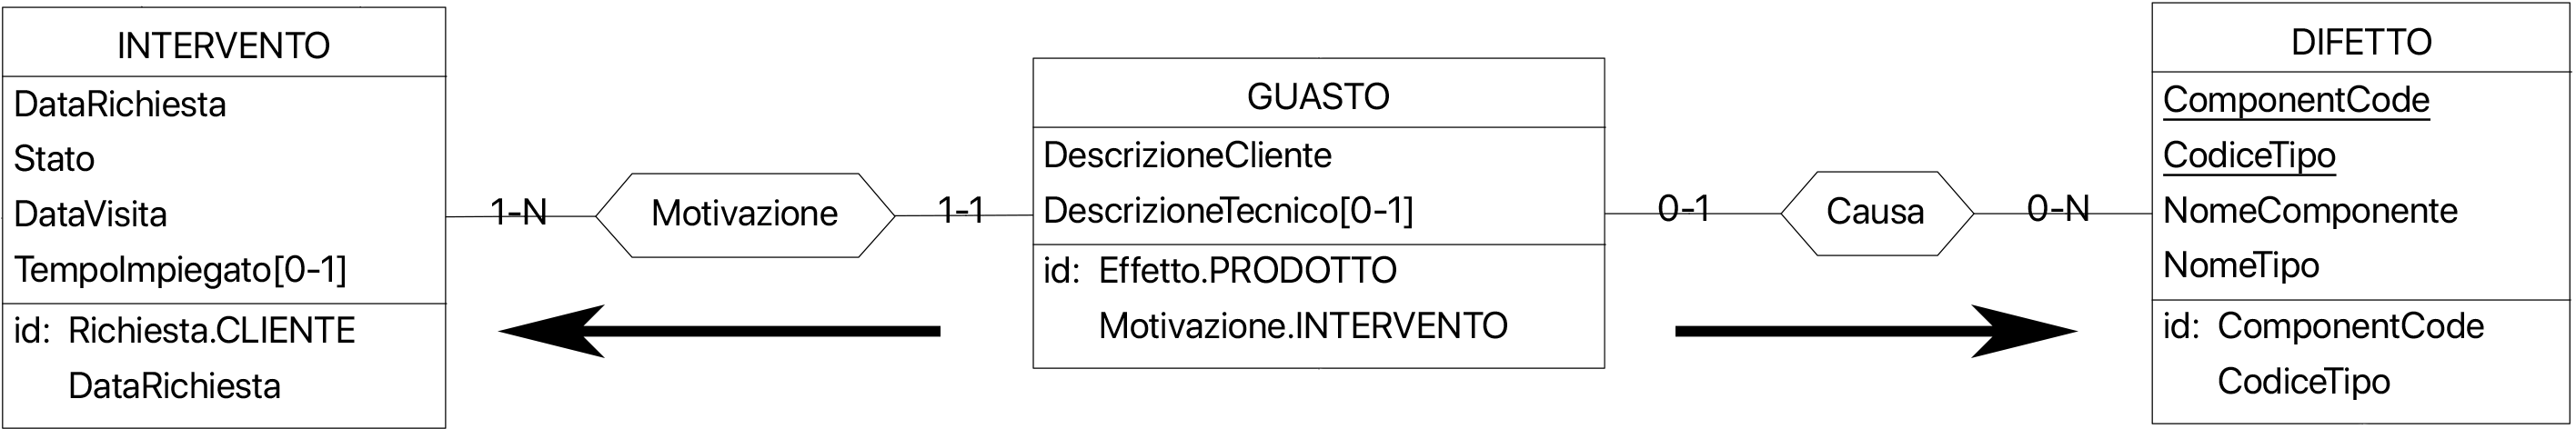
\includegraphics[width=\linewidth]{images/P4.png}
	\caption{Schema di navigazione per l'operazione P4}
\end{figure}

\begin{tabularx}{\linewidth}{X|X|X}
	\hline
	\textbf{Costrutto coinvolto} & \textbf{Accessi} & \textbf{Tipo di Accesso}\\
	\hline
	\hline
	Guasto & 13.220 & L\\
	\hline
	Intervento & 13.220 & L\\
	\hline
	Difetto & 13.220 / 12 = 1.101,667 & L\\
	\hline
	\hline
	TOTALE & \multicolumn{2}{>{\hsize=2\hsize}X}{ 27.541,667 Accessi }\\\hline
	\hline
	\caption{Calcolo degli accessi dell'operazione P4}
\end{tabularx}

\subsection{P5, P6 - I primi cinque ricambi più utilizzati nel riparare i guasti del mese corrente e quelli più costosi nelle riparazioni}

L'operazione P5 non si discosta molto dalle precedenti perché si occupa, una volta ottenuti i guasti del mese, di associarli ai difetti che li hanno causati e poi questi
ai ricambi necessari per ripararli. Una volta fatto, li si raggruppa per ricambio utilizzato e si prendono i primi cinque gruppi che presentano il maggior numero di membri.
L'operazione P6 è identica negli \textit{step} all'operazione P6, anziché però prendere i primi cinque gruppi di ricambi che presentano il maggior numero di membri, vengono
scelti i primi cinque gruppi che presentano una somma dei costi maggiore di quella degli altri. In questo caso si tiene conto del numero dei ricambi utilizzati, ma anche del
loro costo unitario.

\begin{figure}[H]
	\centering
	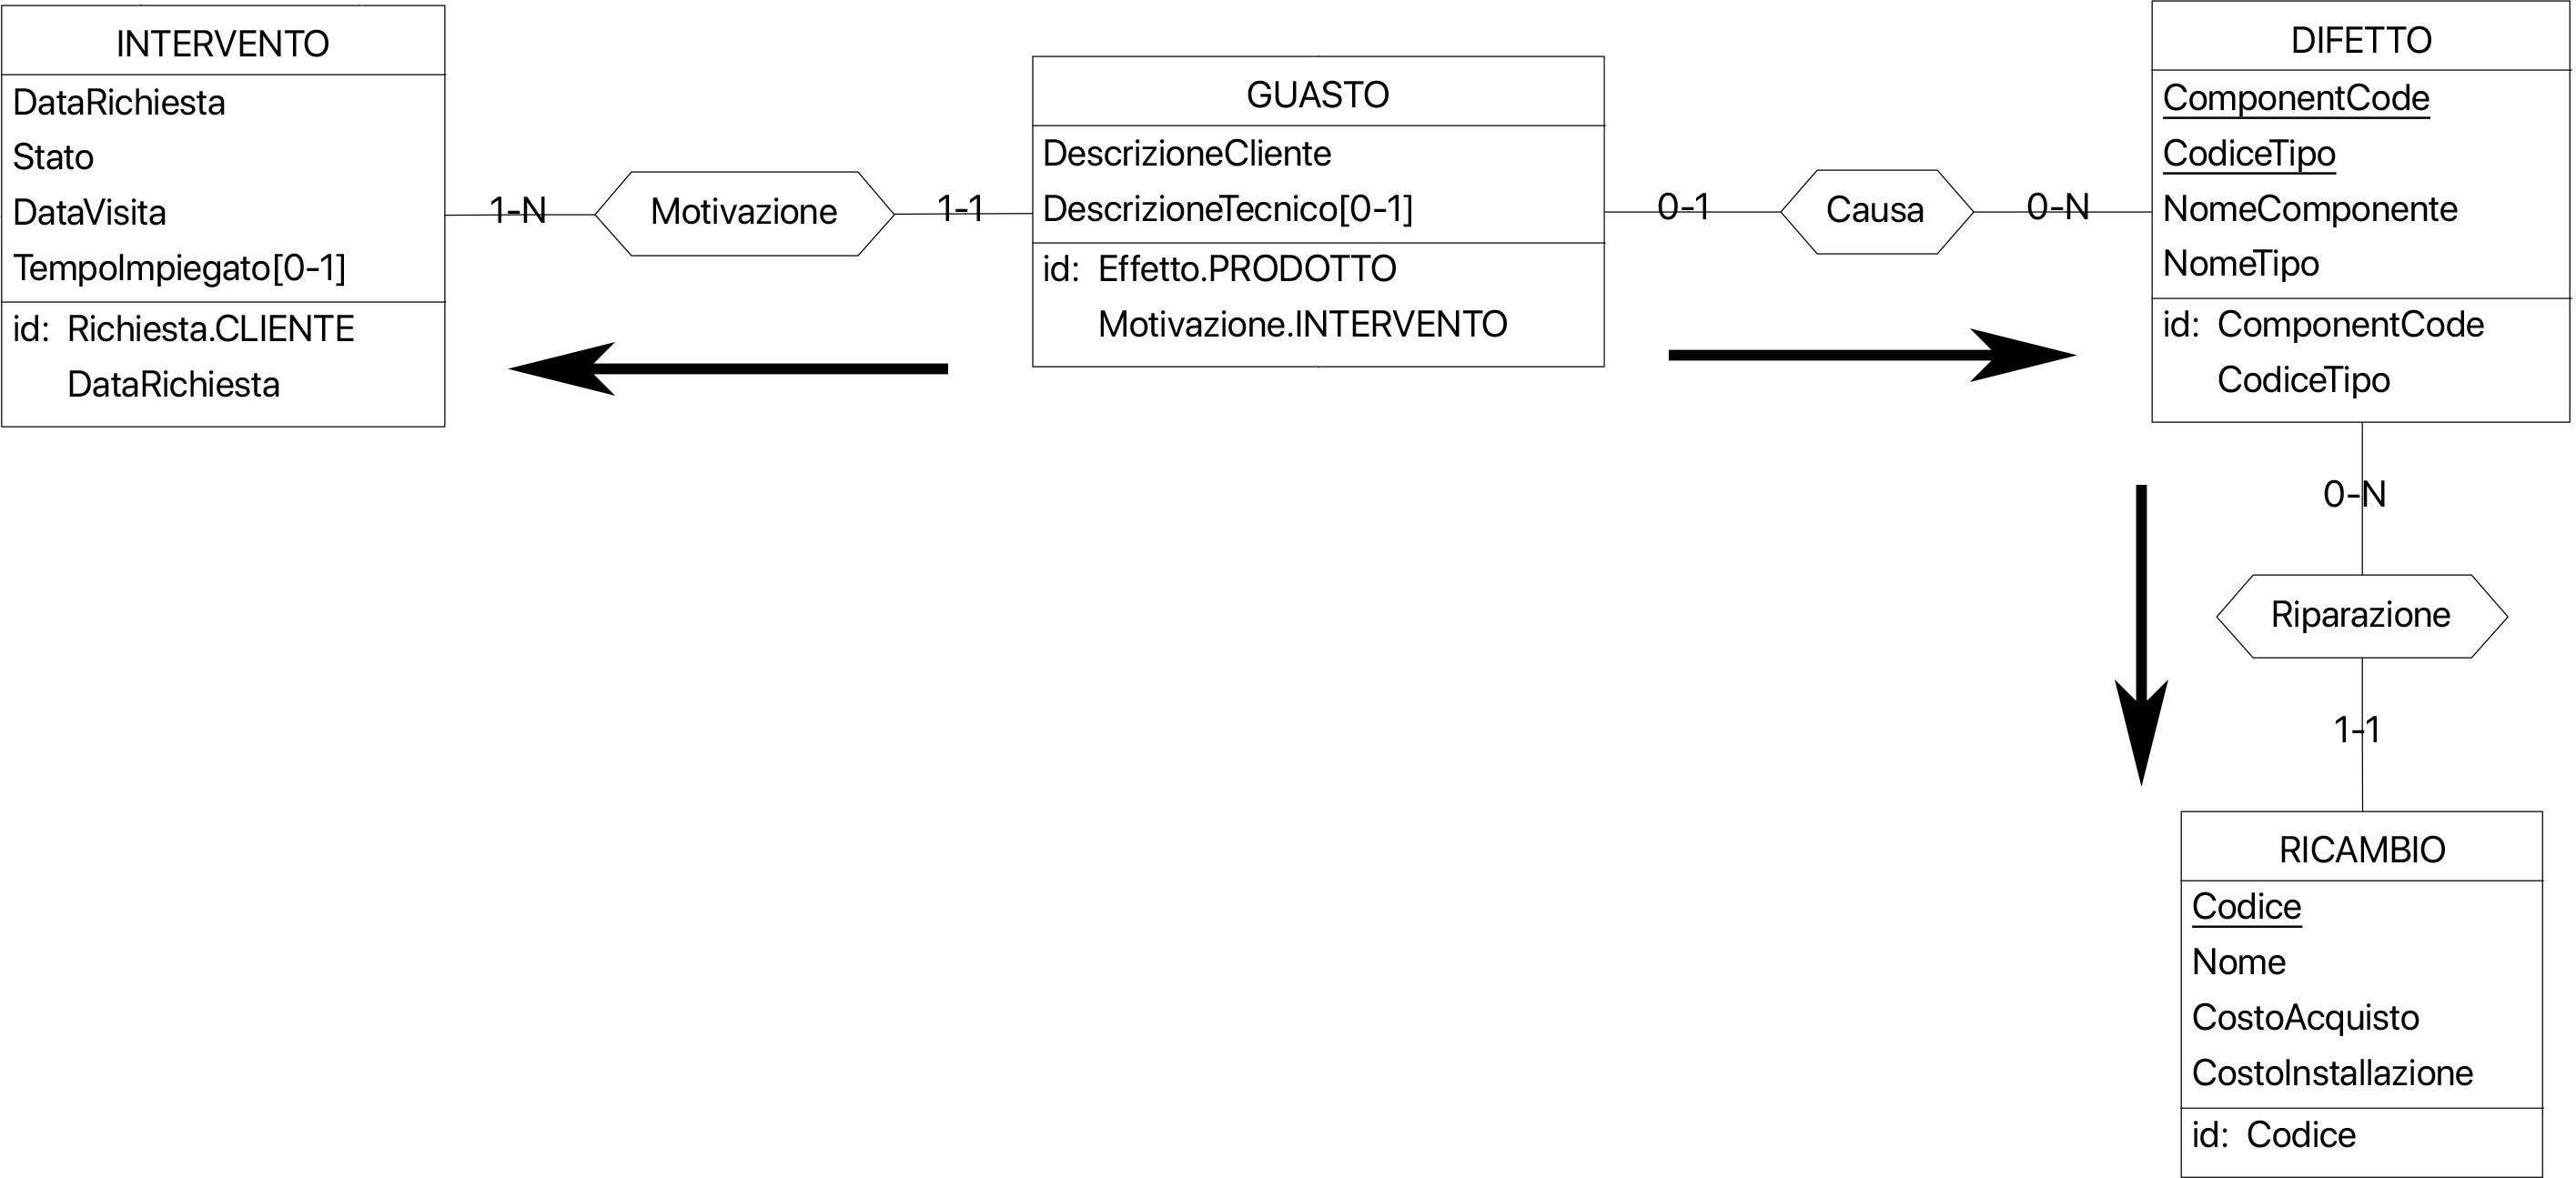
\includegraphics[width=\linewidth]{images/P5-P6.png}
	\caption{Schema di navigazione per le operazioni P5 e P6}
\end{figure}

\begin{tabularx}{\linewidth}{X|X|X}
	\hline
	\textbf{Costrutto coinvolto} & \textbf{Accessi} & \textbf{Tipo di Accesso}\\
	\hline
	\hline
	Guasto & 13.220 & L\\
	\hline
	Intervento & 13.220 & L\\
	\hline
	Difetto & 13.220 / 12 = 1.101,667 & L\\
	\hline
	Ricambio & (75 / 50) * 1.101,667 = 1.652,500  & L\\
	\hline
	\hline
	TOTALE & \multicolumn{2}{>{\hsize=2\hsize}X}{ 29.194,167 Accessi }\\
	\hline
	\hline
	\caption{Calcolo degli accessi delle operazioni P5 e P6}
\end{tabularx}

\subsection{P7 - I primi cinque paesi per numero di guasti di questo mese}

In questa operazione, come nelle precedenti, si prendono in considerazione i guasti del mese corrente, per poi risalire sempre tramite agli interventi che contengono i guasti,
agli operatori che hanno registrato gli interventi e infine attraverso questi ai centri assistenza che hanno accolto la richiesta, identificando la nazione da cui proviene
l'intervento. A questo punto, non resta che raggruppare per nazione e visualizzare i primi cinque gruppi per numero di membri.

\begin{figure}[H]
	\centering
	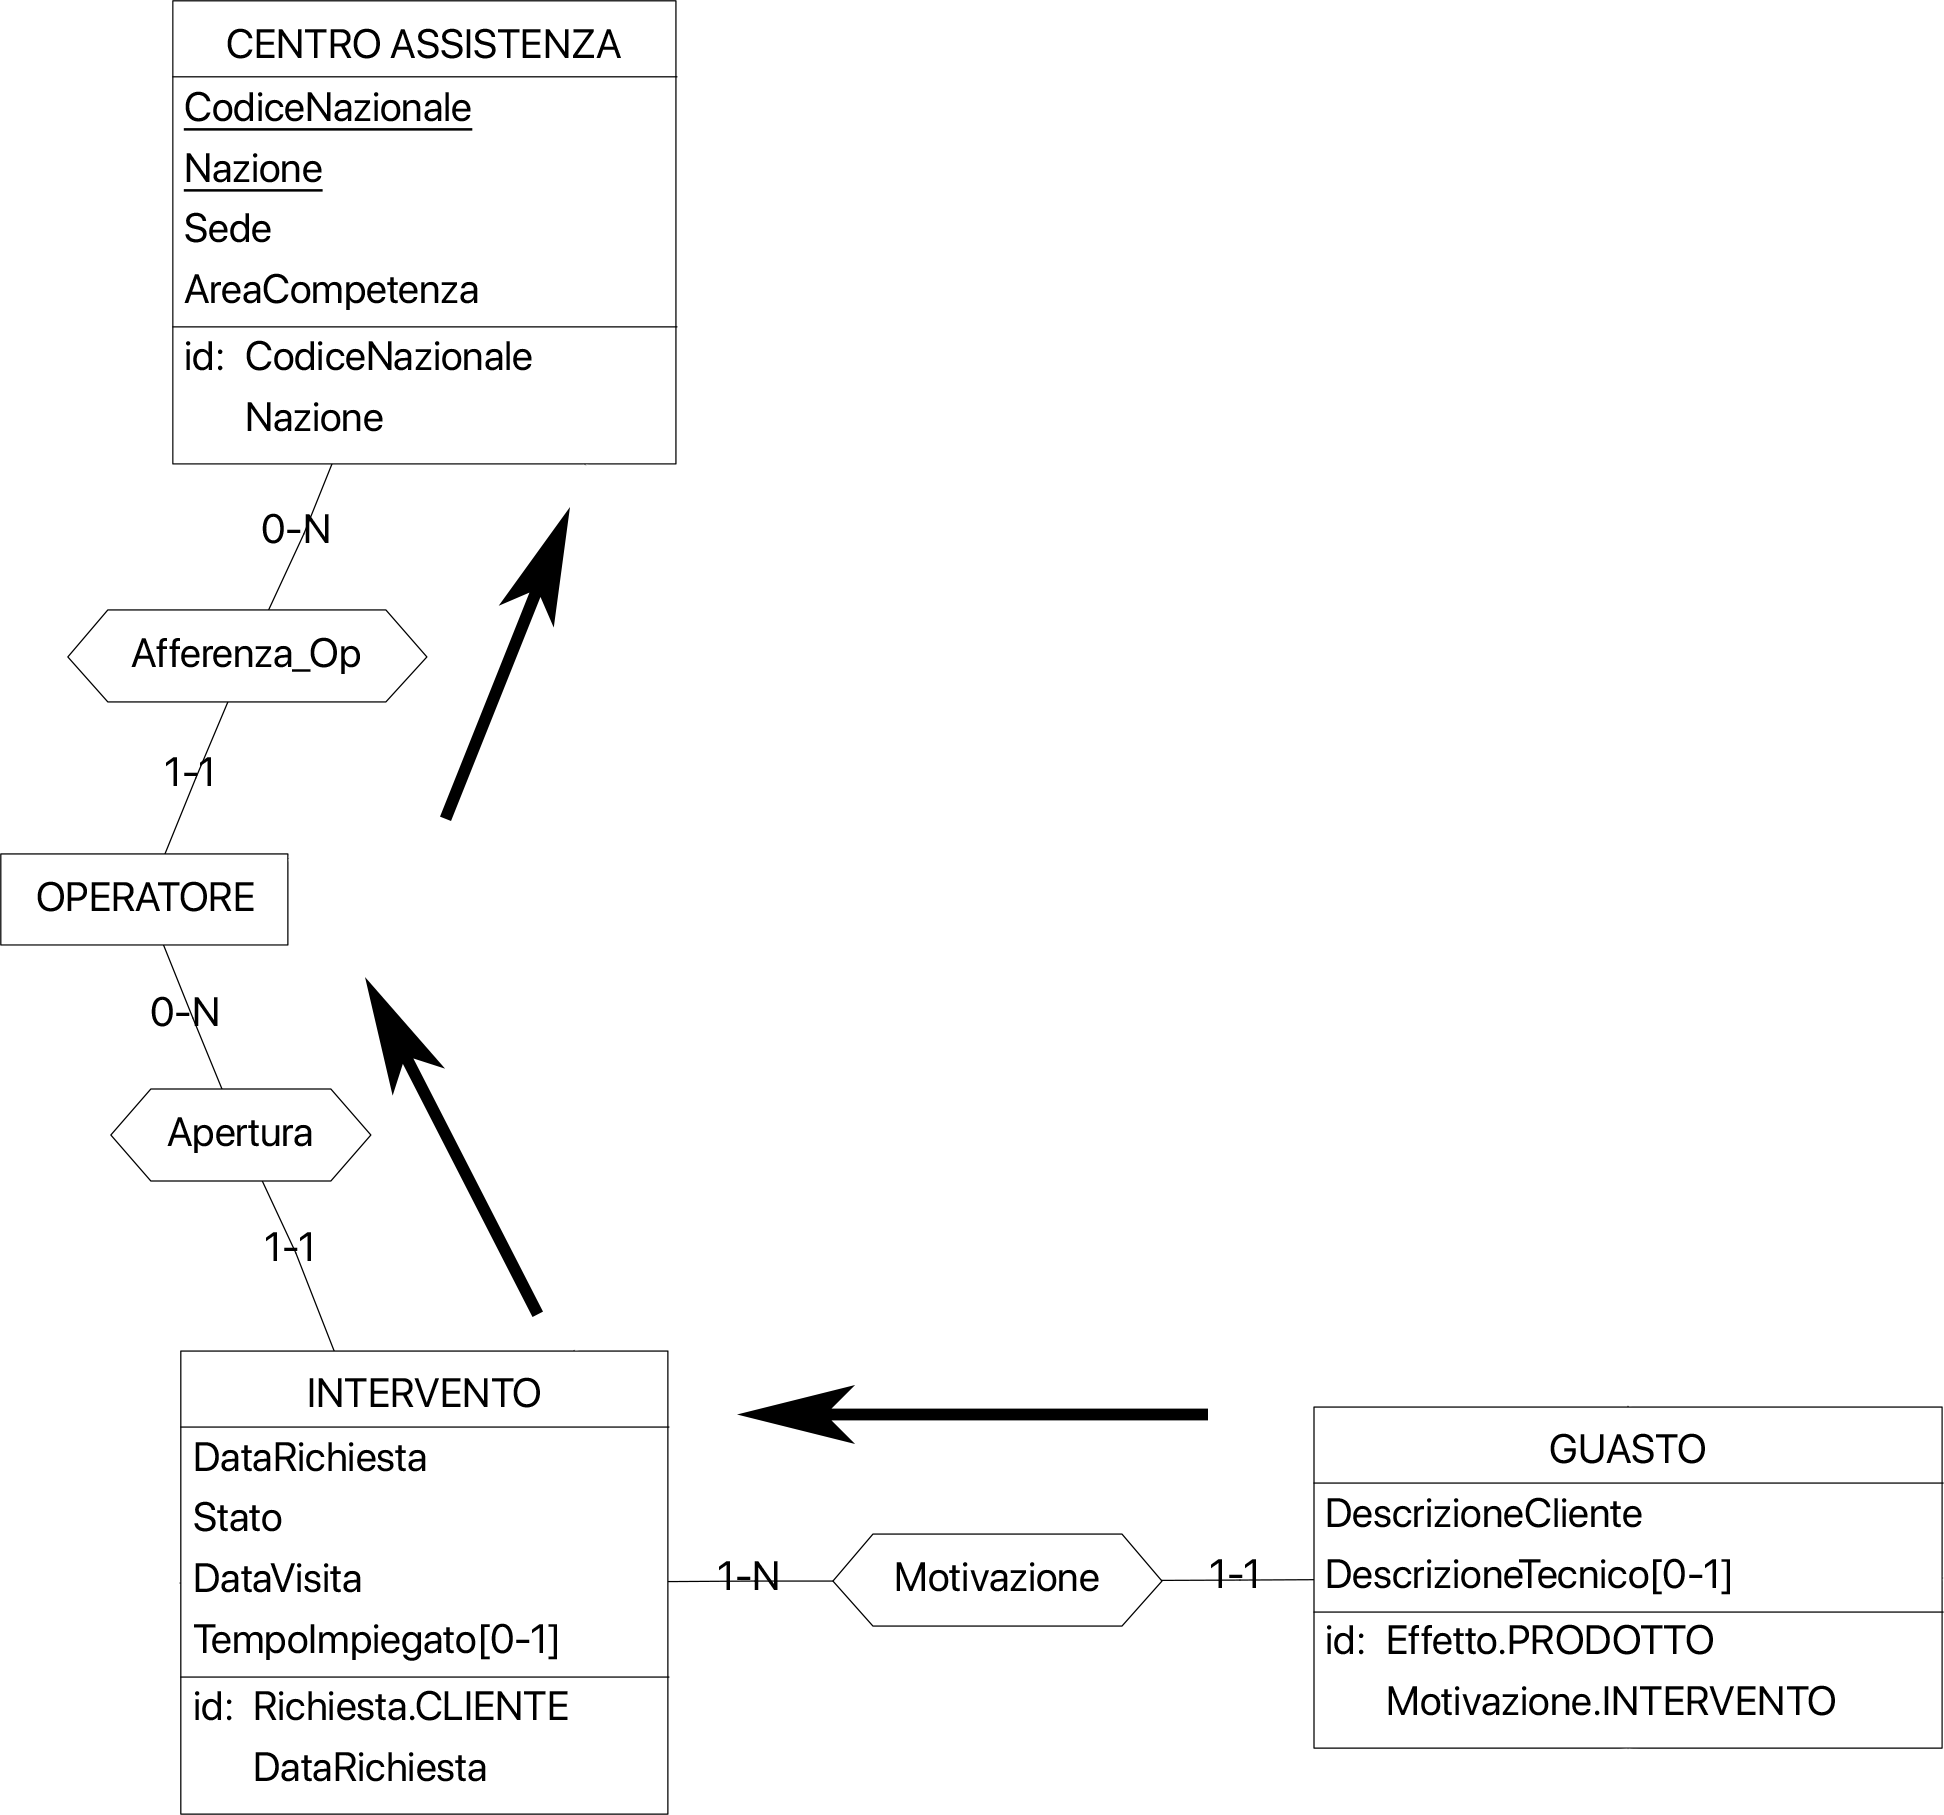
\includegraphics[width=\linewidth]{images/P7.png}
	\caption{Schema di navigazione per l'operazione P7}
\end{figure}

\begin{tabularx}{\linewidth}{X|X|X}
	\hline
	\textbf{Costrutto coinvolto} & \textbf{Accessi} & \textbf{Tipo di Accesso}\\
	\hline
	Guasto & 13.220 & L\\
	\hline
	Intervento & 13.220 & L\\
	\hline
	Operatore & 13.220 / 12 = 1.101,667 & L\\
	\hline
	Centro Assistenza & 1.101,667 & L\\
	\hline
	\hline
	TOTALE & \multicolumn{2}{>{\hsize=2\hsize}X}{ 28.643,334 Accessi }\\\hline
	\hline
	\caption{Calcolo degli accessi dell'operazione P7}
\end{tabularx}

\subsection{P10 - Tempo medio di riparazione di un guasto per tipo di difetto}

Per poter calcolare il tempo medio di riparazione di un guasto occorre per prima cosa accedere all'intervento che lo contiene ed estrarre da questo la data di apertura dell'intervento e quella
di chiusura, così da poter calcolare il tempo impiegato per ripararlo. Dopodiché, per ogni guasto è necessario accedere al difetto che lo ha causato così da poter raggruppare i guasti
per difetto.

\begin{figure}[H]
	\centering
	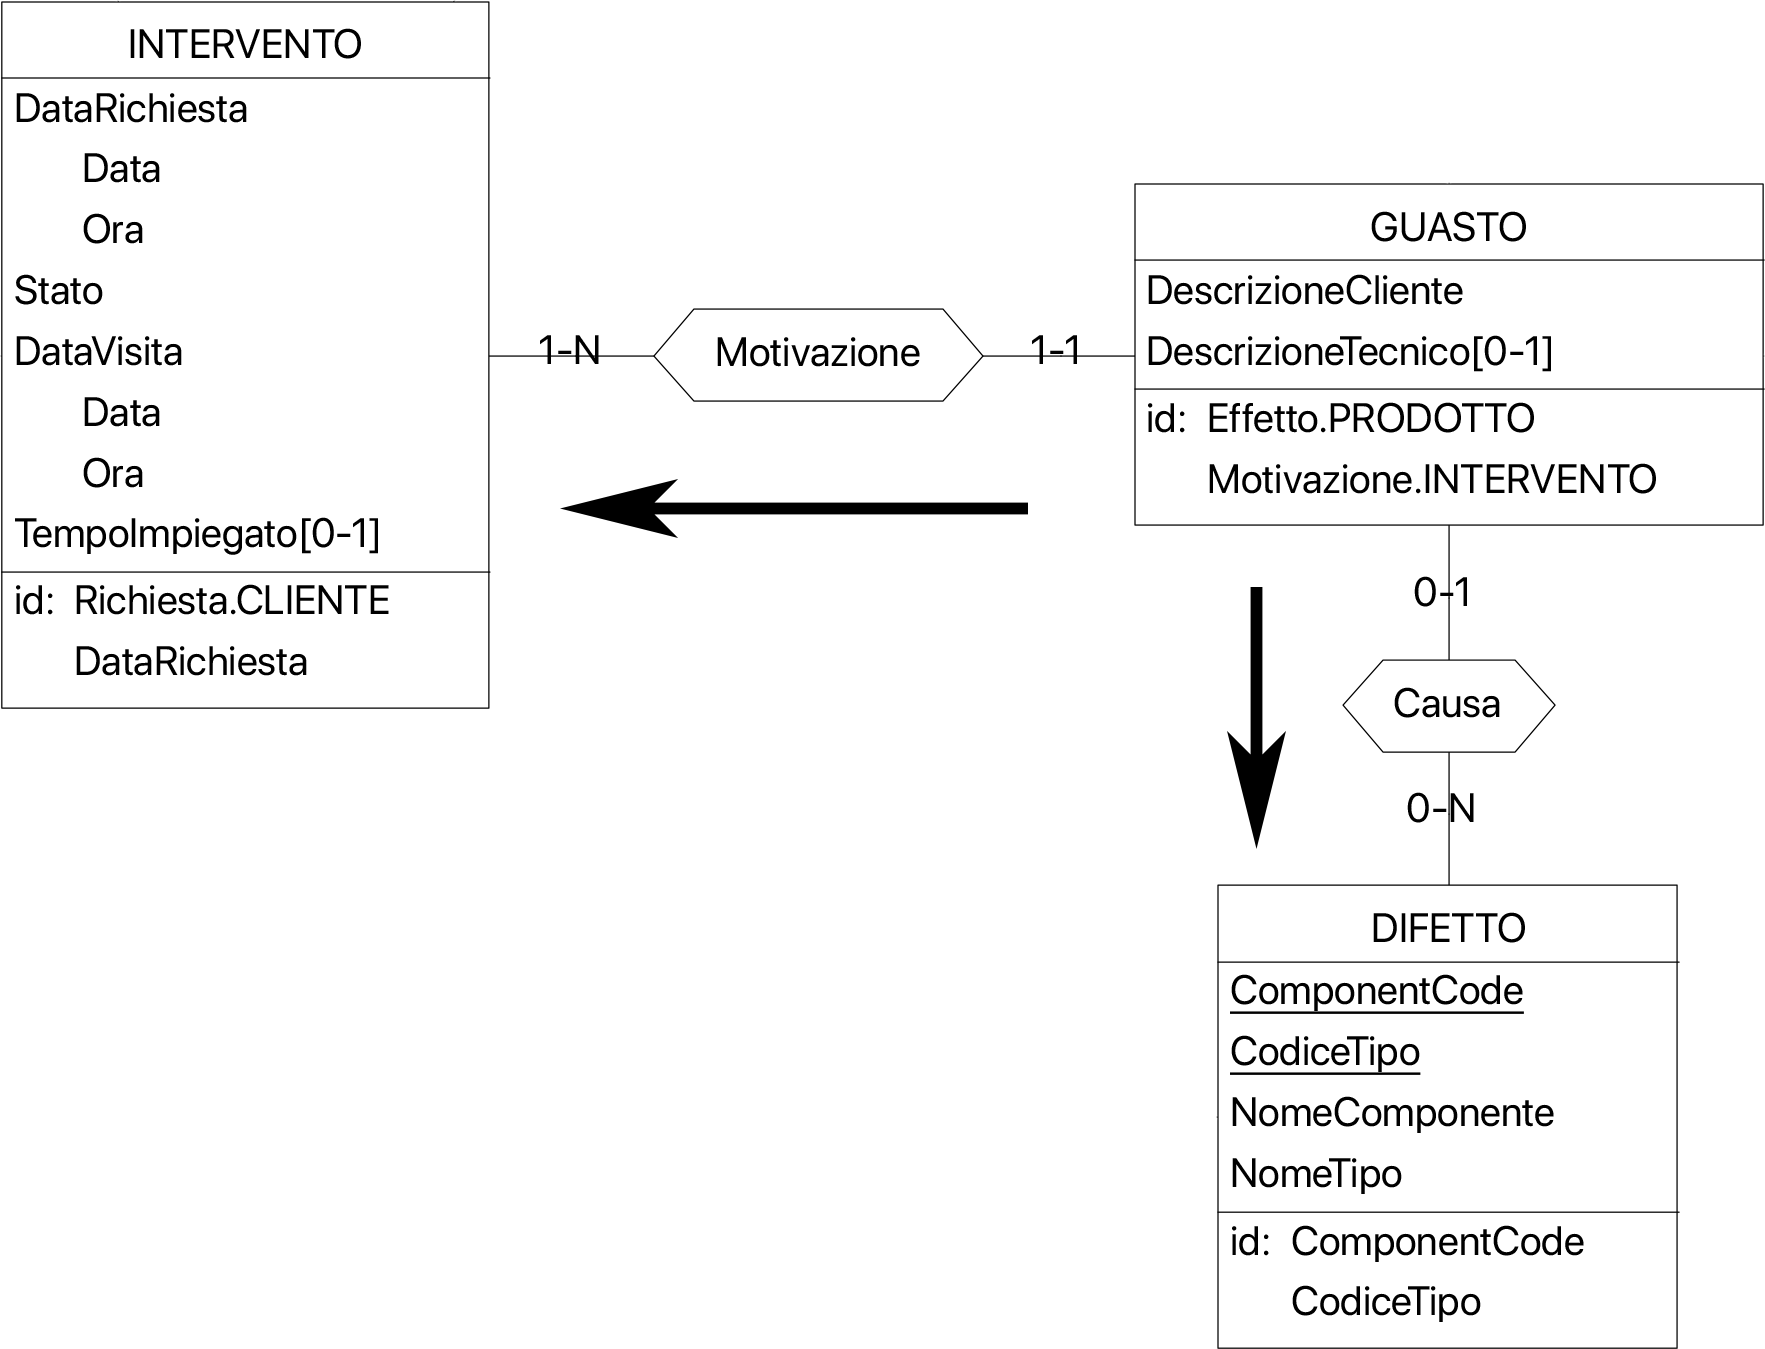
\includegraphics[width=\linewidth]{images/P10.png}
	\caption{Schema di navigazione per l'operazione P10}
\end{figure}

\begin{tabularx}{\linewidth}{X|X|X}
	\hline
	\textbf{Costrutto coinvolto} & \textbf{Accessi} & \textbf{Tipo di Accesso}\\
	\hline
	\hline
	Guasto & 13.220 & L\\
	\hline
	Intervento & 13.220 & L\\
	\hline
	Difetto & 13.220 & L\\
	\hline
	\hline
	TOTALE & \multicolumn{2}{>{\hsize=2\hsize}X}{ 39.660 Accessi }\\\hline
	\hline
	\caption{Calcolo degli accessi dell'operazione T1}
\end{tabularx}

\subsection{V1 - Conteggio di tutti gli interventi aperti nel mese da ciascun operatore}

In questa operazione si suddividono gli interventi che sono stati fatti in questo mese tra i vari operatori sulla base di chi ha aperto quale intervento. Si effettua
poi un raggruppamento per operatore e si contano gli elementi per ciascun sottogruppo.

\begin{figure}[H]
	\centering
	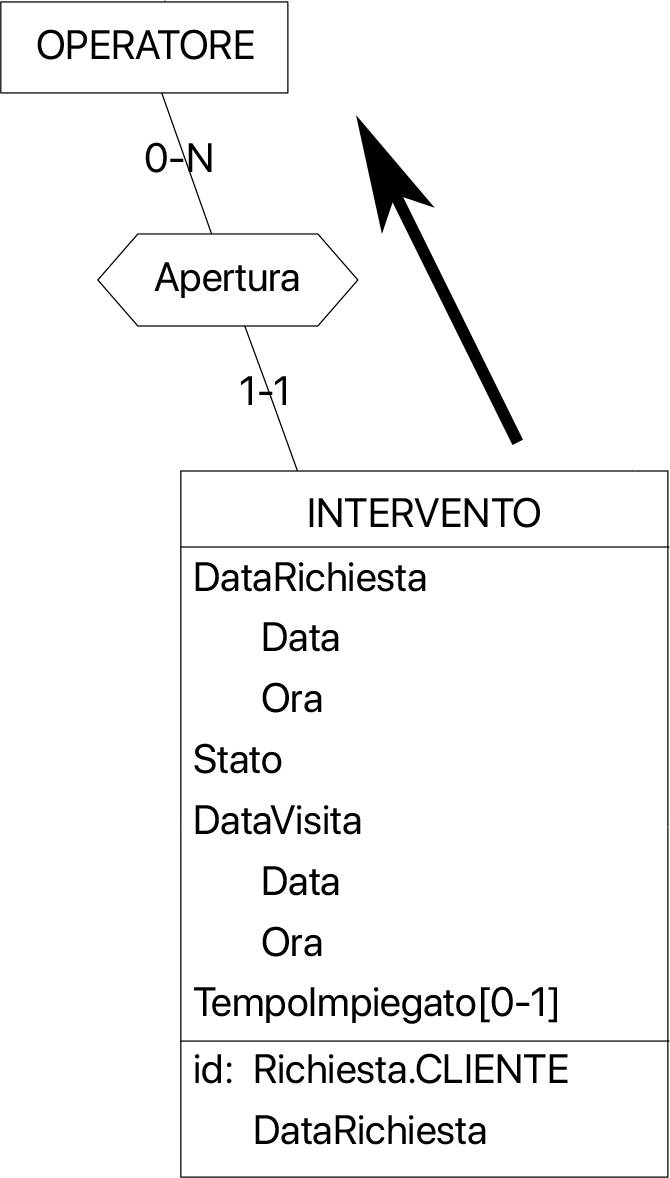
\includegraphics[width=\linewidth]{images/V1.png}
	\caption{Schema di navigazione per l'operazione V1}
\end{figure}

\begin{tabularx}{\linewidth}{X|X|X}
	\hline
	\textbf{Costrutto coinvolto} & \textbf{Accessi} & \textbf{Tipo di Accesso}\\
	\hline
	\hline
	Intervento & 13.200 / 12 = 1.100 & L\\
	\hline
	Operatore & 1.100 & L\\
	\hline
	\hline
	TOTALE & \multicolumn{2}{>{\hsize=2\hsize}X}{ 2.200 Accessi }\\\hline
	\hline
	\caption{Calcolo degli accessi dell'operazione V1}
\end{tabularx}

\subsection{V2, V3 - Conteggio di tutti gli interventi chiusi nel mese e tempo medio di riparazione per ciascun tecnico}

Queste due operazioni non sono per nulla dissimili dalla precedente, se non per il fatto che i dipendenti coinvolti sono i tecnici e non gli operatori e,
se l'operazione V2 è identica nei passaggi alla precedente, l'operazione V3 sceglie come criterio da visualizzare per ciascun gruppo non tanto il numero di
elementi dello stesso ma la media dei tempi necessari per la risoluzione dei problemi che il tecnico ha sistemato.

\begin{figure}[H]
	\centering
	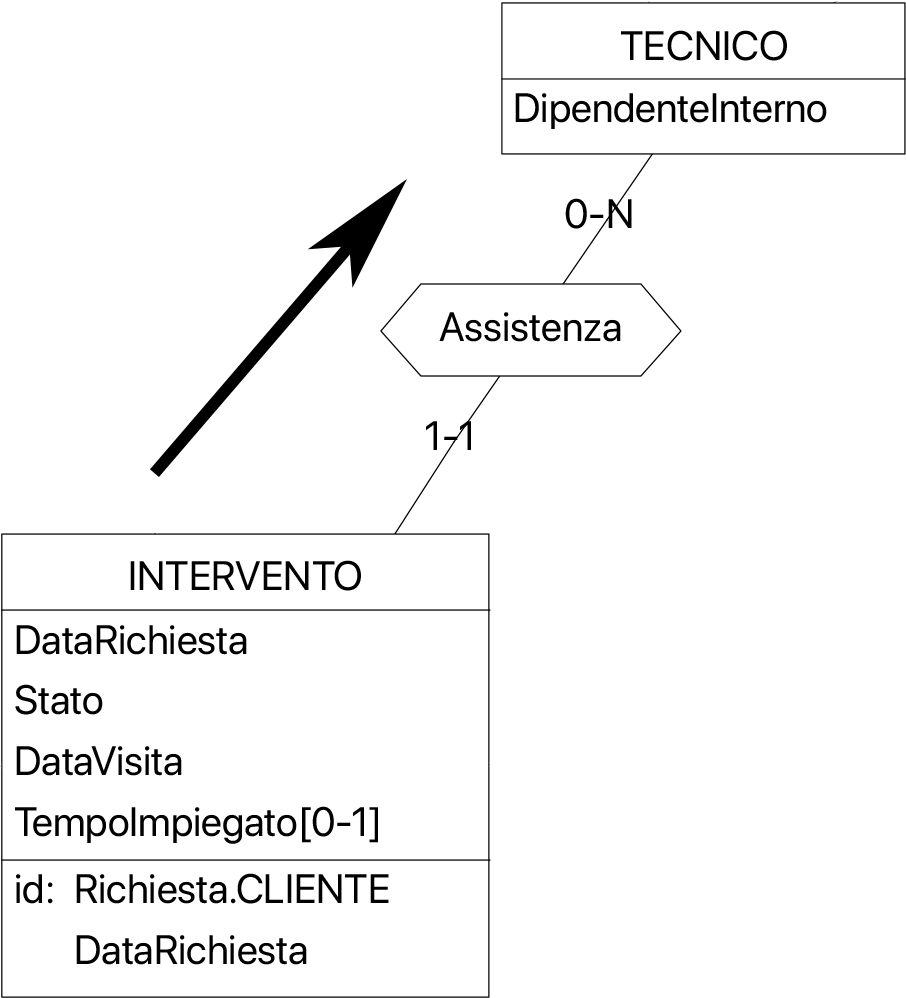
\includegraphics[width=\linewidth]{images/V2-V3.png}
	\caption{Schema di navigazione per le operazioni V2 e V3}
\end{figure}

\begin{tabularx}{\linewidth}{X|X|X}
	\hline
	\textbf{Costrutto coinvolto} & \textbf{Accessi} & \textbf{Tipo di Accesso}\\
	\hline
	\hline
	Intervento & 13.200 / 12 = 1.100 & L\\
	\hline
	Tecnico & 13.200 / 12 = 1.100 & L\\
	\hline
	\hline
	TOTALE & \multicolumn{2}{>{\hsize=2\hsize}X}{ 2.200 Accessi }\\\hline
	\hline
	\caption{Calcolo degli accessi delle operazioni V2 e V3}
\end{tabularx}

\subsection{V4 -  Distanza temporale media tra ricezione della chiamata e visita del tecnico per centro assistenza}

Questa operazione raggruppa gli interventi per centro assistenza che li ha creati e per ogni gruppo calcola la media del tempo di vita di un intervento, dalla sua apertura
dopo una chiamata alla sua chiusura dopo la visita di un tecnico.

\begin{figure}[H]
	\centering
	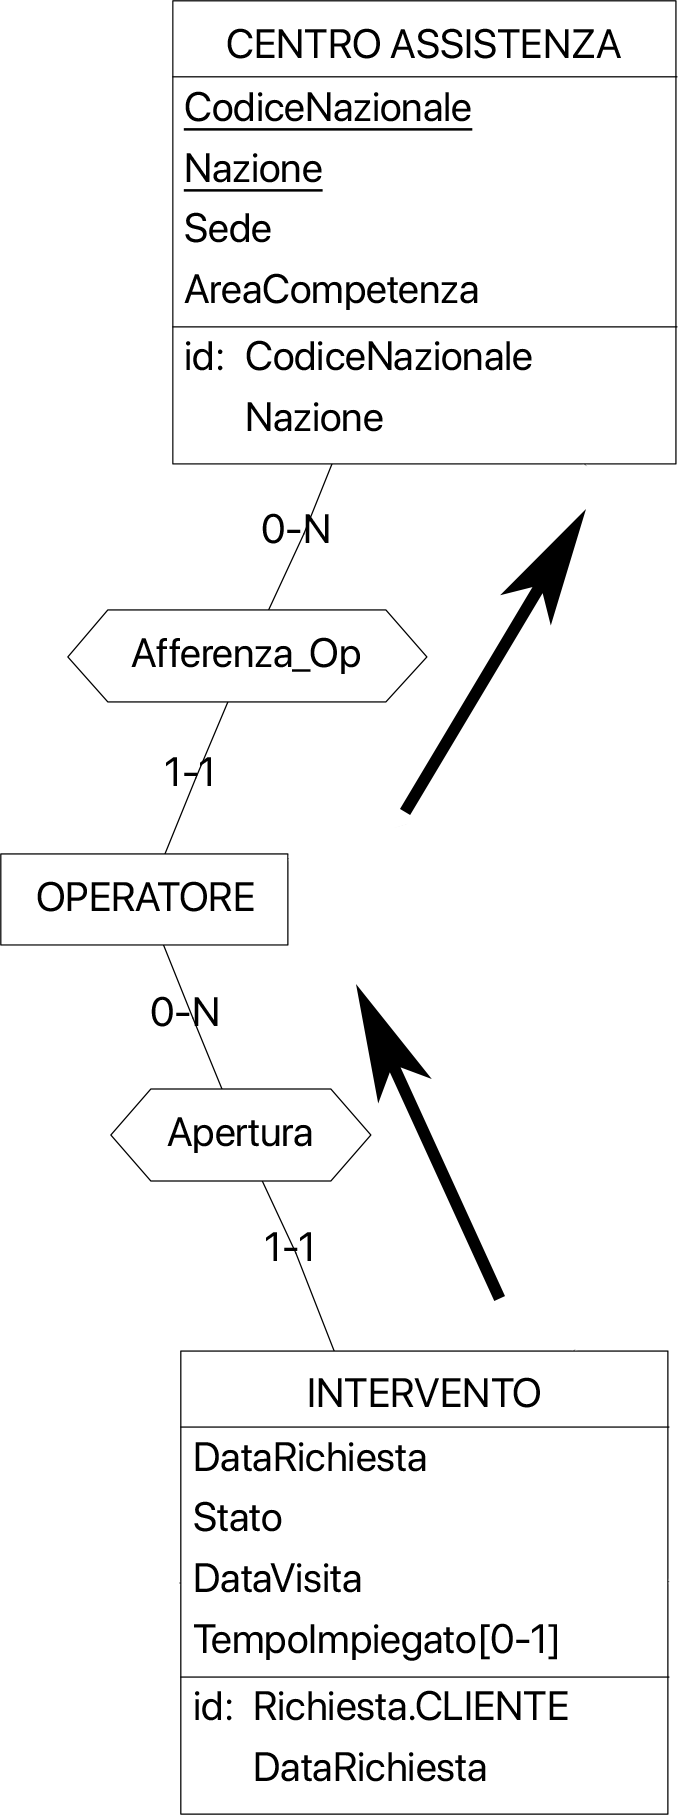
\includegraphics[width=\linewidth]{images/V4.png}
	\caption{Schema di navigazione per l'operazione V4}
\end{figure}

\begin{tabularx}{\linewidth}{X|X|X}
	\hline
	\textbf{Costrutto coinvolto} & \textbf{Accessi} & \textbf{Tipo di Accesso}\\
	\hline
	\hline
	Intervento & 13.200 & L\\
	\hline
	Operatore & 13.200 & L\\
	\hline
	Centro Assistenza & 13.200 & L\\
	\hline
	\hline
	TOTALE & \multicolumn{2}{>{\hsize=2\hsize}X}{ 39.600 Accessi }\\\hline
	\hline
	\caption{Calcolo degli accessi dell'operazione V4}
\end{tabularx}

\section{Raffinamento dello schema concettuale}

Per rendere traducibile lo schema "\textit{Entity-Relationship}" in uno schema relazionale, occorre effettuare alcune modifiche allo schema stesso
cercando di mantenere quanto più possibile alta la fedeltà dei concetti rappresentati.

\subsection{Eliminazione delle gerarchie}

La rimozione della gerarchia che discende direttamente da persona è, delle due presenti, la più semplice. L'entità persona, volta esclusivamente a fattorizzare
i campi comuni, non ha nessuna utilità pratica oltre quella citata all'interno dello schema. Si procede perciò ad eliminarla con un collasso verso il basso,
duplicando i campi "Nome" e "Cognome" per le entità "Cliente" e "Dipendente". Per la seconda gerarchia, quella che origina da "Dipendente", si decide anche in questo
caso di effettuare un collasso verso il basso perché, osservando le principali operazioni individuate, nessuna richiede l'accesso alla totalità dei dipendenti tutti assieme,
anzi, al contrario. Ben tre operazioni vengono effettuate su una specifica categoria di dipendenti in maniera indipendente dagli altri e se decidessimo di creare un'unica
relazione con tutti i dipendenti finirebbero per aumentare il loro costo in termini di "\textit{I/O}". Inoltre, in entrambe le gerarchie, non abbiamo nessun tipo di associazione
che figura legata all'entità padre, perciò nessuno vi farà mai accesso e non saranno presenti dopo la modifica associazioni duplicate.

\subsection{Eliminazione di attributi multipli}

Nello schema è presente un solo attributo multiplo, la categoria di interesse dei progettisti, che come sappiamo può essere anche più di una. Si decide perciò di isolarla in
un entità a sé stante e legarla a "Progettista" mediante un'associazione "uno a molti". Essa sarà costituita dal nome della categoria e da un codice che la identifica univocamente.
Allo stesso modo, ogni prodotto, che appartiene ad una categoria, avrà la propria categoria di appartenenza specificata mediante il codice identificativo della categoria stessa.

\subsection{Scelta delle chiavi primarie}

Lo schema "\textit{Entity-Relationship}" evidenzia già in maniera chiara gli attributi che concorrono ad essere potenziali chiavi primarie e si decide di utilizzare quelle
indicate senza effettuare ulteriori modifiche. Molte chiavi infatti sono già dei semplici codici e perciò non è necessario semplificarle. Le chiavi più complesse che appaiono nello
schema sono quelle di "Intervento" e "Guasto". La prima entità è individuata da un "Cliente" e da una data. "Cliente" però è identificato univocamente dal solo numero di telefono,
facendo perciò in modo che un intervento sia identificato da una data e un numero di telefono. Conseguentemente, un guasto viene identificato da un numero di telefono, una data e i
due codici identificativi di prodotto. Entrambi questi due identificatori perciò non appaiono essere troppo complessi e in particolar modo l'identificatore di guasto presenta alcuni
attributi - "DataIntervento", "PNC" - utilizzati in alcune operazioni che coinvolgono i guasti, permettendo di averli già disponibili senza effettuare ulteriori accessi ad altre relazioni,
diminuendo i costi legati a quelle specifiche operazioni.

\begin{figure}[H]
	\centering
	\includegraphics[width=\linewidth]{images/Refined.png}
	\caption{Schema E/R dopo i raffinamenti individuati nei paragrafi precedenti}
\end{figure}

\section{Analisi delle ridondanze}

Le associazioni che figurano come ridondanti nello schema sono due: "Analisi", tra "Progettista" e "Guasto", e "Proprietà", tra "Cliente" e "Prodotto". Queste due associazioni
condividono il fatto che nessuna delle due è utilizzata delle principali operazioni individuate e in particolar modo, nessuna delle due è particolarmente utile ai nostri scopi.\newline
L'associazione "Analisi", infatti, dovrebbe tenere conto di tutti i possibili guasti che sono di interesse per ciascuno dei progettisti, che però provocherebbe non poche ridondanze
a livello di record per nessun utilizzo. Vero è che abbiamo indicato che non tutti i progettisti sono interessati a visionare tutti i guasti, ma filtrare questi dati può essere effettuato
anche senza la presenza esplicita di questa associazione, tanto più che abbiamo indicato le operazioni di creazione delle statistiche come "\textit{batch}", quindi da eseguire in
un momento diverso, possibilmente antecedente, rispetto a quello in cui i progettisti accederanno ai dati. Sarà poi quando un progettista richiederà la visualizzazione dei dati che
essi saranno filtrati sulla base delle categorie di suo interesse.\newline
Per quanto riguarda invece "Proprietà", pur essendo vero che il cliente effettua una telefonata per un elettrodomestico che possiede, non abbiamo alcun interesse ad utilizzare mai
questa nozione. Il fatto che sia presente il cliente associato ad un intervento è perché necessitiamo di sapere presso chi mandare il tecnico per la riparazione. Quale che sia il prodotto
che possiede è a noi indifferente, poiché non ci interessano statistiche di vendita o similari. Nell'estremo caso volessimo risalire, per un dato cliente, a quali elettrodomestici
ha comprato - e gli si sono necessariamente guastati - possiamo sempre farlo attraverso "Intervento" e "Guasto".\newline
Attributi ridondanti eliminabili già presenti nello schema "\textit{Entity-Relationship}" non sono presenti. Per semplificare le operazioni da effettuare su base mensile, si può pensare di importare la data di apertura dell'intervento all'interno dell'entità "Guasto", cosa che però viene già effettuata in quanto "Intervento" è parte integrante della chiave di "Guasto" e perciò
non è richiesta alcuna modifica ulteriore.\newline
Un'altra modifica che si può effettuare è importare la nazione in cui l'intervento viene aperto all'interno dell'entità "Intervento" stessa. Questo attributo "Nazione" sarebbe perciò
la nazione di appartenenza del centro assistenza a cui l'operatore che riceve la chiamata fa capo, in quanto si suppone che ogni cliente che chiama venga diretto al centro assistenza 
adeguato alla sua zona di residenza secondo l'azienda. Questa introduzione di ridondanza porterebbe all'aumento del costo dell'operazione O1, ma ad una diminuzione del costo di P7.

\begin{tabularx}{\linewidth}{X|X|X}
	\title{Operazione O1}
	\hline
	\textbf{Costrutto coinvolto} & \textbf{Accessi} & \textbf{Tipo di Accesso}\\
	\hline
	\hline
	Intervento & 1 & S\\
	\hline
	Cliente & 1 & S\\
	\hline
	Guasto & 13.220 / 13.200 = 1,002 & S\\
	\hline
	Prodotto & 13.220 / 13.200 = 1,002 & S\\
	\hline
	\hline
	TOTALE & \multicolumn{2}{>{\hsize=2\hsize}X}{ 8,008 Accessi }\\\hline
	\hline
	\caption{Calcolo degli accessi delle operazioni O1 e O2}
\end{tabularx}

\section{Traduzione di entità e associazioni in relazioni}

\section{Schema finale}

\section{Traduzione delle operazioni in SQL}

\chapter{Progettazione dell'applicazione}

\end{document}